%%  本模板推荐以下方式编译: xelatex
%%     1. 文件默认的编码为 UTF-8 对于windows,请选用支持UTF-8编码的编辑器。
%%   2. 若是模板有什么问题,请及时与我们取得联系,Email:latexstudio@qq.com。
%%   3. 可以到  https://ask.latexstudio.net 提问
%%   4. 请安装 最新版本的 TeXLive 地址:
%%   http://mirrors.ctan.org/systems/texlive/Images/texlive.iso

\documentclass[12pt,a4paper]{nmmcm}
\usepackage{ctex}
\usepackage{gbt7714}
\usepackage{float}
\usepackage{graphicx}
\usepackage{booktabs,colortbl}
\usepackage{xcolor}
\usepackage{tikz}
\usepackage{indentfirst}
\mcmsetup{CTeX = true,
        tcn ={\xiaowuhao 1001 }(\textcolor{red}{\textit{1103}}), problem = A,
        sheet = true, titleinsheet = false, keywordsinsheet = true,
        titlepage = true, abstract = true}
\usepackage{xurl}
\setmainfont{Times New Roman}
\setmonofont[
    Path=fonts/,
    UprightFont = *-Regular,
    BoldFont = *-Bold,
    ItalicFont = *-Italic
]{UbuntuMono}
\usepackage{lipsum}


\usepackage{paralist}
\let\itemize\compactitem
\let\enditemize\endcompactitem
\let\enumerate\compactenum
\let\endenumerate\endcompactenum
\let\description\compactdesc
\let\enddescription\endcompactdesc

\setlength{\parindent}{2em} 
\setlength\abovedisplayskip{5pt}
\setlength\belowdisplayskip{-8pt}
\setlength{\parskip}{0.1em}

\newcommand\wordc[1]{\textbf{#1}}
\renewcommand{\appendixtocname}{附\quad录}
\renewcommand{\appendices}{\hspace{-2em}{\sanhao\HEI {\bf 附~~~录}}}
\colorlet{tableheadcolor}{gray!25} % Table header colour = 25% gray
\newcommand{\headcol}{\rowcolor{tableheadcolor}}

\title{TRS}
\date{}

\usepackage[font=small,labelfont={bf,sf},tableposition=top]{caption}


\begin{document}
\author{杨在洲}
\begin{abstract}


%abstract---------------
{\fangsong\xiaosihao
\setlength{\parindent}{2em}
社会消费品零售总额是衡量人们消费水平的重要指标,也是国民经济体系中的一个重要指标。
预测2022年疫情损失的社会消费品零售总额,可以将其应用于的对整体经济损失的一个关键要素。

首先通过对以往月度统计数据进行STL季节性分解,得到时间序列的季节波动情况。
然后先对原时间序列进行一阶差分,再对差分后序列进行季节差分,得到平稳的时间序列。再通过季节性ARIMA模型进行参数估计,并
得到2022年未受到疫情干预的预测值。接着利用2020年前的数据建立ARIMA模型,得到2020年未受疫情影响的预测值。通过2020年
预测值和实际值,建立在疫情干预下的干预分析模型。继而应用该模型得到2022年在疫情干预下的
预测值。最终结合ARIMA模型的预测值,预测2022年社会消费品零售总额的损失。
并通过R语言进行建模和计算以及绘图。
}









\begin{keywords}
{\song\xiaosihao
社会消费品零售总额,季节性ARIMA模型, 时间序列分析,干预分析模型}
\end{keywords}


\end{abstract}
\maketitle
\renewcommand{\contentsname}{\centerline{\sanhao\bfseries\HEI 目\quad 录}}
%\thispagestyle{empty}
%{\song\xiaosihao
\tableofcontents
%}


\newpage
\setcounter{page}{1}
\pagestyle{fancy}
\song\xiaosihao


\section{模型假设}
\begin{enumerate}
  \item 模型假设一:2022年3月起疫情对社会消费品零售总额产生干预
  \item 模型假设二:2022年疫情对经济的干预情况与2020年相同
  \item 模型假设三:2022年四月为损失最严重的一个月,五月起逐步恢复
\end{enumerate}

\section{主要符号与说明}

%tab1
\begin{table}[h!]
  \centering
  \small
  \begin{tabular}{p{60pt}<{\centering}|p{60pt}<{\centering}p{180pt}<{\raggedright}}
   \hline
   \headcol 序号 & 符号 & 符号说明 \\
   \hline
    1 & $X_t$ & 社会消费品零售总额的时间序列 \\
    2 & $T_t$ & 趋势因子时间序列 \\
    3 & $S_t$ & 季节因子时间序列 \\
    4 & $R_t$ & 随机误差因子时间序列 \\
    5 & $\hat{X}_t$ & 对\(X_t\)一阶差分后的时间序列 \\
    6 & $\epsilon_t$ & 白噪声序列 \\
    7 & $p$ & 自回归阶数 \\
    8 & $q$ & 移动平均阶数 \\
    9 & $X'$ & 对\(\hat{X}_t\)季节差分后的时间序列 \\
    10 & $B$ & 滞后算子 \\
    11 & $lag$ & 滞后阶数 \\
    12 & $\omega$ & 疫情干预系数 \\
    13 & $Z_t$ & 疫情发生后产生损失的时间序列 \\
    $\cdots$ & $\cdots$\\
    \hline
  \end{tabular}
  %\caption{符号与说明}
  \label{symbol}
\end{table}

\section{数据分析}
\subsection{数据来源}
本次建模采用的数据为2012年1月起至2022年4月的月度数据,\href{http://www.gov.cn/shuju/hgjjyxqk/xiangqing/tcg.html}{来自国家统计局}。
由于在 1-2 月只有总和的数据,在此简单假设两月每天的零售总额相同,
则一月份总额在 1-2 月总和的占比在闰年和平年的占比分别为
\(51.7\% \; ,52.5\%\) ,得到表格如下:
% Table generated by Excel2LaTeX from sheet 'Sheet1'
\begin{table}[H]
  \centering
  \caption{社会商品零售总额月度数据(单位: 亿元)}
  \resizebox{\textwidth}{!}{
    \begin{tabular}{c|ccccccccccc}
          & 2012  & 2013  & 2014  & 2015  & 2016  & 2017  & 2018  & 2019  & 2020  & 2021  & 2022 \\
          \hline
    1     & 17171.0  & 19866.4  & 21563.2  & 25216.7  & 26984.3  & 30453.8  & 31151.7  & 34712.0  & 27390.6  & 36641.8  & 37957.3  \\
    2     & 16497.6  & 17943.4  & 20717.5  & 22775.8  & 25926.0  & 27505.9  & 29930.1  & 31352.0  & 24739.2  & 33095.0  & 36468.7  \\
    3     & 15650.2 & 17641.2 & 19800.6 & 22722.8 & 25114.1 & 27863.7 & 29193.6 & 31725.7 & 26449.9 & 35484.1 & 34233.1 \\
    4     & 15603.1 & 17600.3 & 19701.2 & 22386.7 & 24645.8 & 27278.5 & 28541.9 & 30586.1 & 28177.8 & 33152.6 & 29483.1\\
    5     & 16714.8 & 18886.3 & 21249.8 & 24194.8 & 26610.7 & 29459.2 & 30359.1 & 32955.7 & 31972.8 & 35945.1 &  \\
    6     & 16584.9 & 18826.7 & 21166.4 & 24280.3 & 26857.4 & 29807.6 & 30841.6 & 33878.1 & 33525.9 & 37585.8 &  \\
    7     & 16314.9 & 18513.2 & 20775.8 & 24338.8 & 26827.4 & 29609.8 & 30733.7 & 33073.3 & 32202.5 & 34925.1 &  \\
    8     & 16658.9 & 18886.2 & 21133.9 & 24893.4 & 27539.6 & 30329.7 & 31542.3 & 33896.3 & 33570.6 & 34394.9 &  \\
    9     & 18226.6 & 20653.3 & 23042.4 & 25270.6 & 27976.4 & 30870.3 & 32005.4 & 34494.9 & 35294.7 & 36833.0 &  \\
    10    & 18933.8 & 21491.3 & 23967.2 & 28278.9 & 31119.2 & 34240.9 & 35534.4 & 38104.3 & 38576.5 & 40453.9 &  \\
    11    & 18476.7 & 21011.9 & 23474.7 & 27937.3 & 30958.5 & 34108.2 & 35259.7 & 38093.8 & 39514.2 & 41043.2 &  \\
    12    & 20334.2 & 23059.7 & 25801.3 & 28634.6 & 31757.0 & 34734.1 & 35893.5 & 38776.7 & 40566.0 & 41268.9 &  \\
    \end{tabular}}%
  \label{tab:addlabel}%
\end{table}%

根据表格中所给数据,由于2022年三月份时吉林,上海等各省市集中爆发疫情,因此选择2022年2月份以前的数据作为训练集,以时间为横轴,绘出折线图如下:
\begin{figure}[H] %H为当前位置,!htb为忽略美学标准,htbp为浮动图形
  \centering %图片居中
  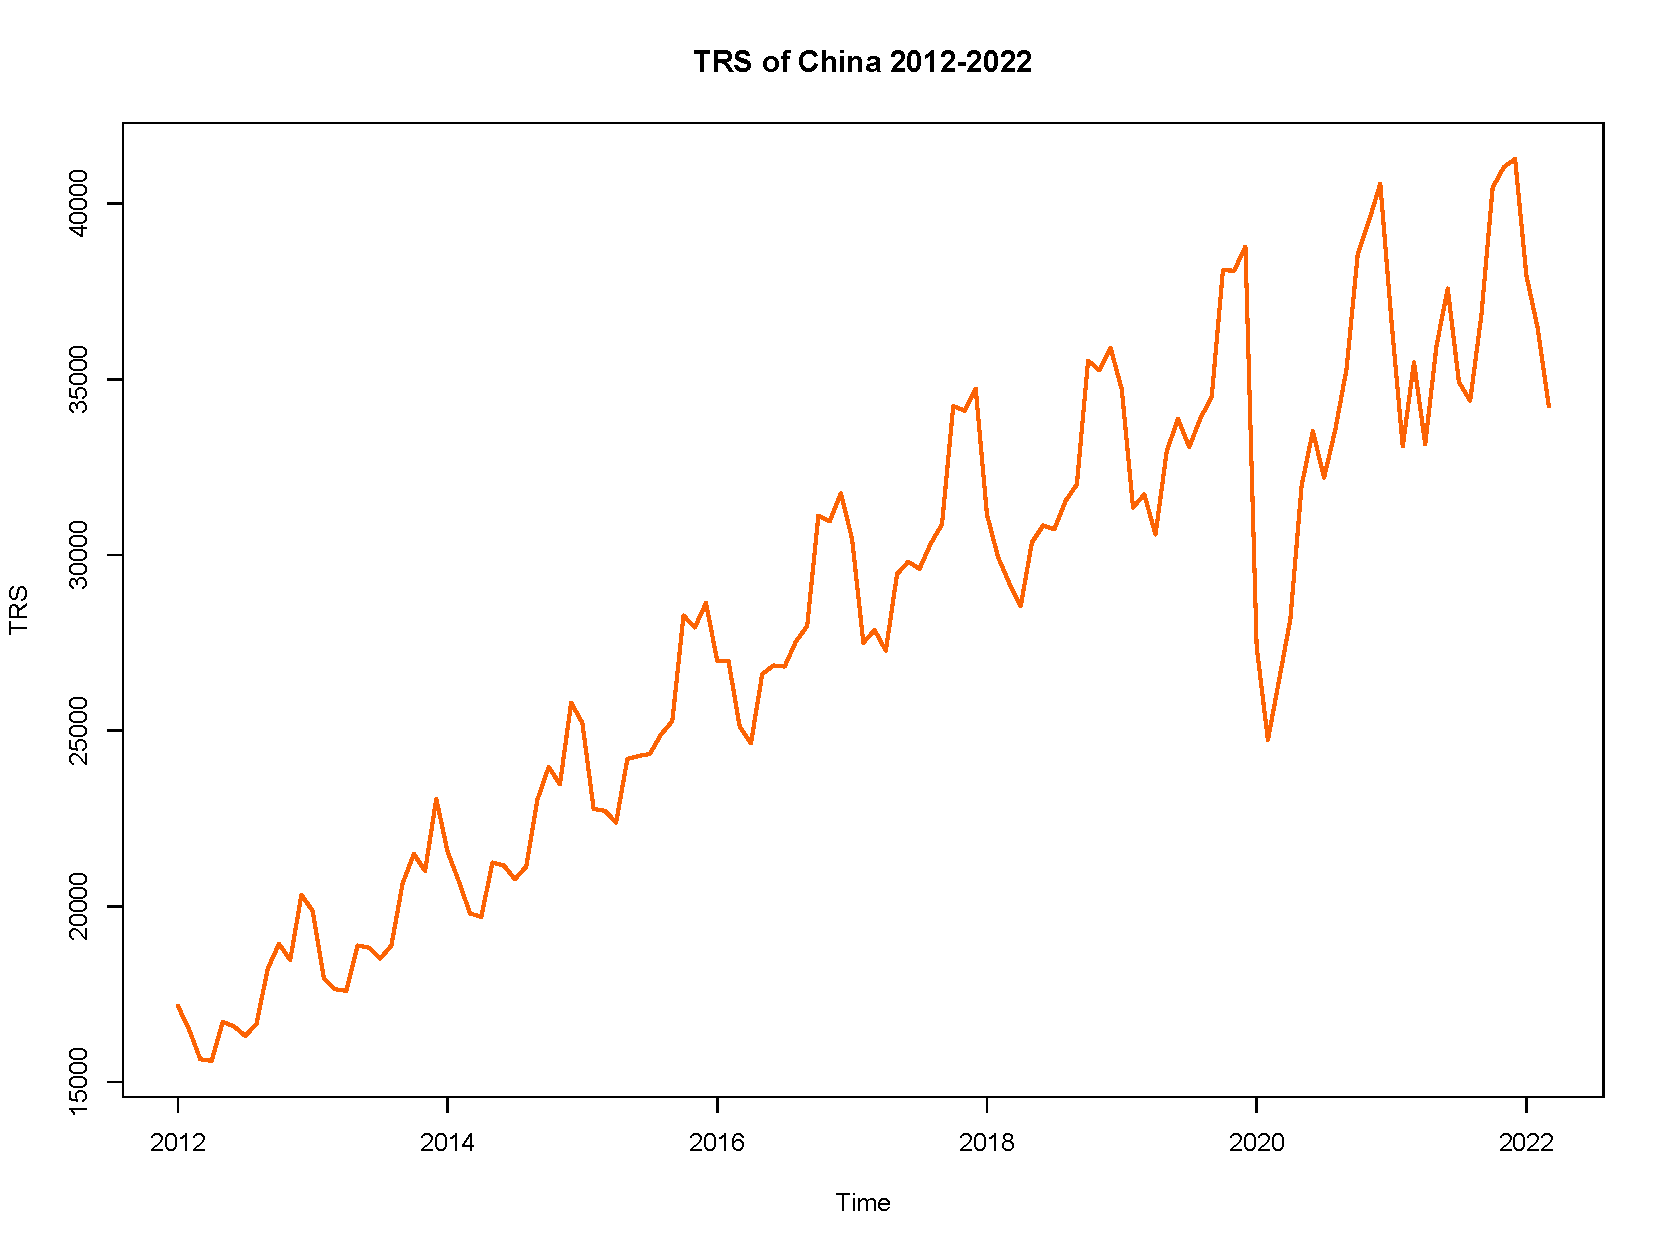
\includegraphics[width=0.6\textwidth]{Raw_TRS.pdf} %插入图片,[]中设置图片大小,{}中是图片文件名
  \caption{社会消费品零售总额2012-2022} %最终文档中希望显示的图片标题
  \label{TRS} %用于文内引用的标签
  \end{figure} 
\subsection{季节性分解}
可以看出社会消费品零售总额的变化呈明显的季节波动,并且呈现逐年上升趋势,
所以考虑通过STL算法用Loess平滑化后将时间序列数据分解为
趋势因子(trend compoents)\(T_t\),季节因子(season compoents)\(S_t\),和随机误差因子(remmainder compoents)\(R_t\)\cite{STL}\nocite{yang2022estimating}:
\begin{equation}
  X_t = T_t + S_t + R_t
\end{equation}

得到分解图如下:
\begin{figure}[H] %H为当前位置,!htb为忽略美学标准,htbp为浮动图形
  \centering %图片居中
  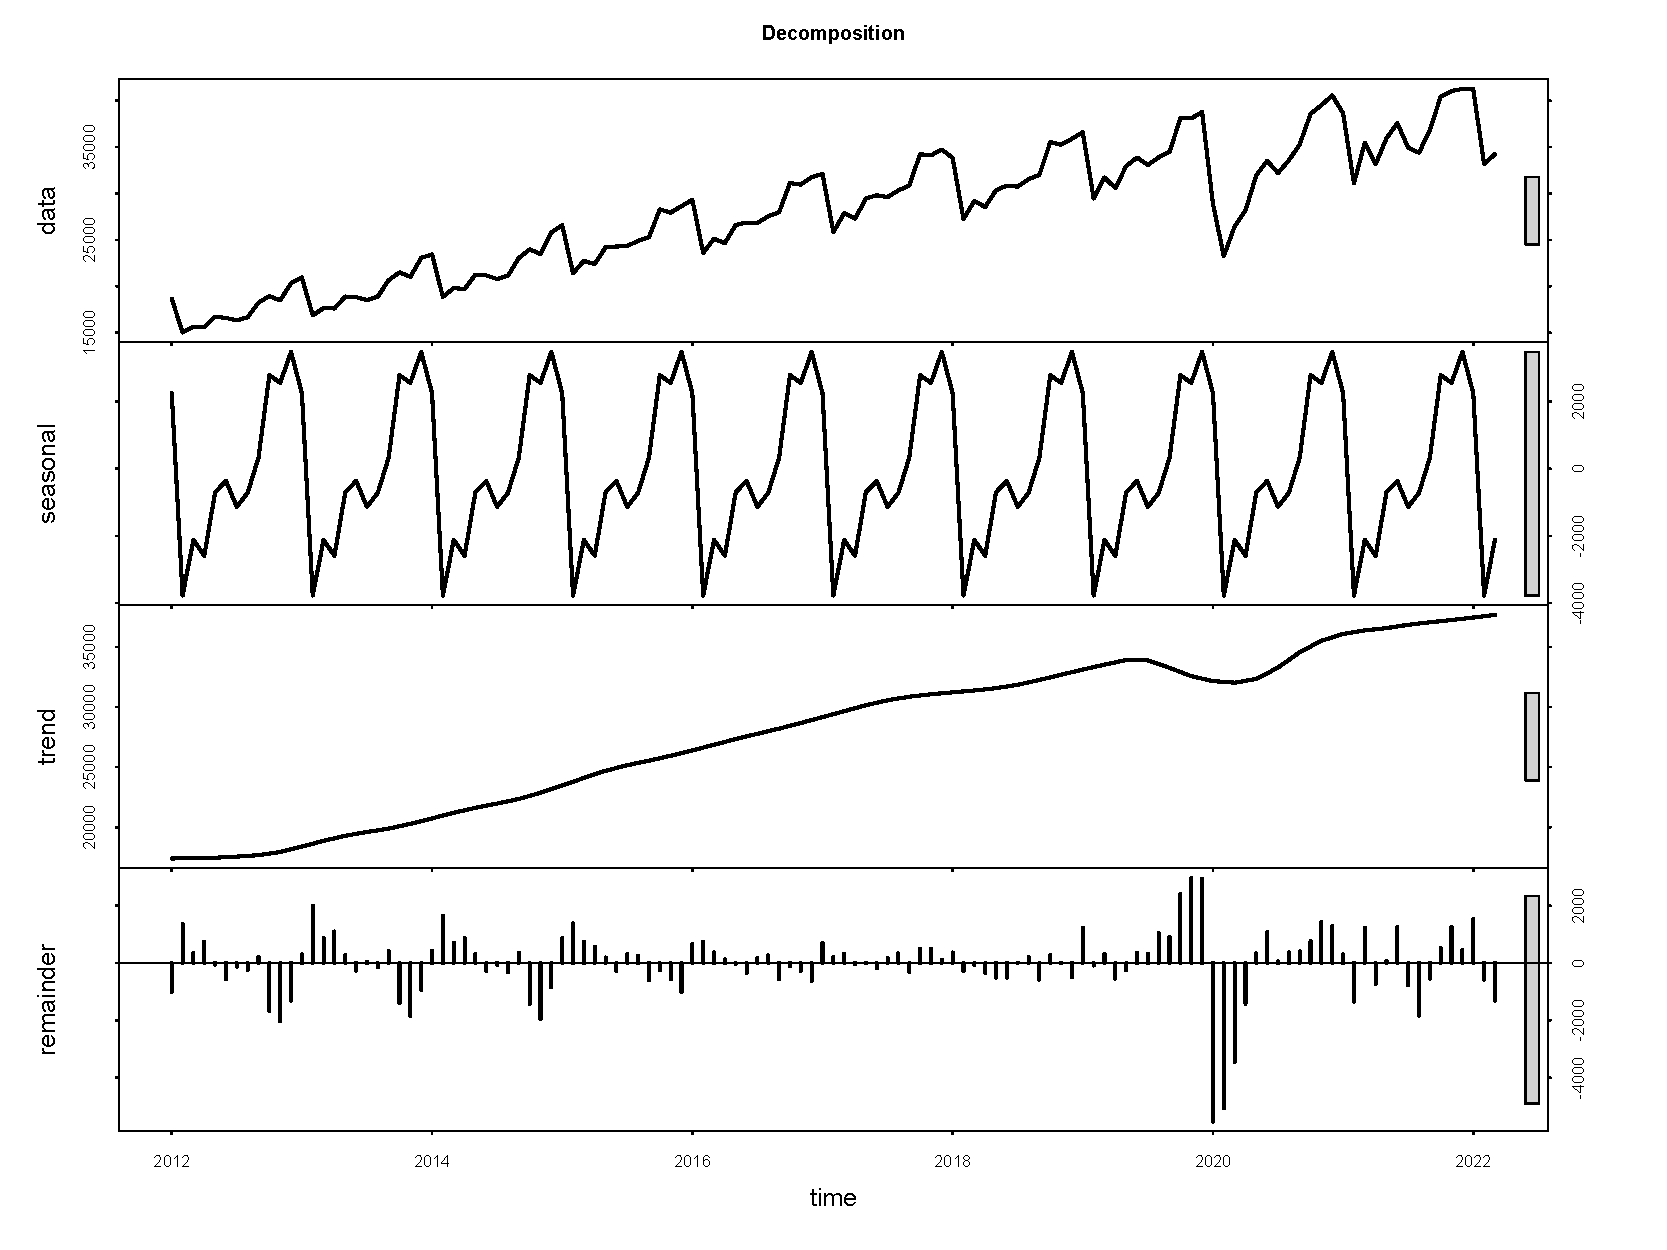
\includegraphics[width=1\textwidth]{decompose.pdf} %插入图片,[]中设置图片大小,{}中是图片文件名
  \caption{按加法模型分解后} %最终文档中希望显示的图片标题
  \label{decompose} %用于文内引用的标签
\end{figure} 

从趋势因子来看,总体趋势稳步提升直至2020疫情爆发前,到2020年末基本恢复
正常发展水平,持续稳步发展到2022年2月。
 \par 从季节因子来看,在春节前,即年末12月份,消费达到顶峰,之后逐步下降至四月份到达最低点,之后开始逐步攀升
直至12月份。
\section{ARIMA模型建立}

\subsection{数据检验}

\subsubsection*{数据平稳性检验}
若时间序列\(X_t\)满足如下条件:

  (1) 均值\(E ( X_t ) = \mu \),均值\(\mu\)是与时间\(t\)无关的常数

  (2) 方差\(Var(X_t) = \sigma^2\),方差\(\sigma\)是与时间\(t\)无关的常数

  (3) 协方差\(Cov(X_t,X_{t+k}) = \gamma^2\),协方差只与间隔\(t\)有关  

  则称时间序列\(X_t\)是平稳的。

由表\ref{TRS}中可明显看出均值随时间\(t\)增长,可以猜测原序列应为非平稳序列。
采用\(ADF\)检验原序列的平稳性,\(ADF\) 检验通过一下三个模型检验:
\begin{equation}
  \begin{aligned}
  &\Delta X_t = \delta X_{t-1} + \sum_{i=1}^{m}\beta_i X_{t-i} + \epsilon_t \\
  &\Delta X_t =\alpha + \delta X_{t-1} + \sum_{i=1}^{m}\beta_i X_{t-i} + \epsilon_t \\
  &\Delta X_t =\alpha +\beta_t+ \delta X_{t-1} + \sum_{i=1}^{m}\beta_i X_{t-i} + \epsilon_t
  \end{aligned}
\end{equation}

三个模型原假设都是\(H_0 : \delta = 0\).若拒绝\(H_0\)则为平稳序列,否则为非平稳序列。
通过\(ADF \)临界值表判断是否接受\(H_0\)\nocite{Ruey}

为验证猜想对原序列做\(ADF\)检验,得到结果如下:
% Table generated by Excel2LaTeX from sheet 'Sheet1'
\begin{table}[htb]
  \centering
  \caption{Add caption}
    \begin{tabular}{lr}
    \multicolumn{2}{c}{ Augmented Dickey-Fuller Test} \\
    \hline
    Lag Order: & 1 \\
    Dickey-Fuller: & 0.3394\\
    P Value  & 0.7218 \\
    \end{tabular}%
  \label{tab:ADF_raw}%
\end{table}%

由于\(p-value > 0.05 \)所以无法拒绝原假设,因此原序列是非平稳的。
为了将原序列转化为平稳序列处理,因为从图\ref{TRS}看出原序列应该
有随时间线性增加的趋势,考虑对原序列做一阶差分\cite{Rob},得到新序列\(\hat{X}_t\)如下图:
\begin{figure}[H] %H为当前位置,!htb为忽略美学标准,htbp为浮动图形
  \centering %图片居中
  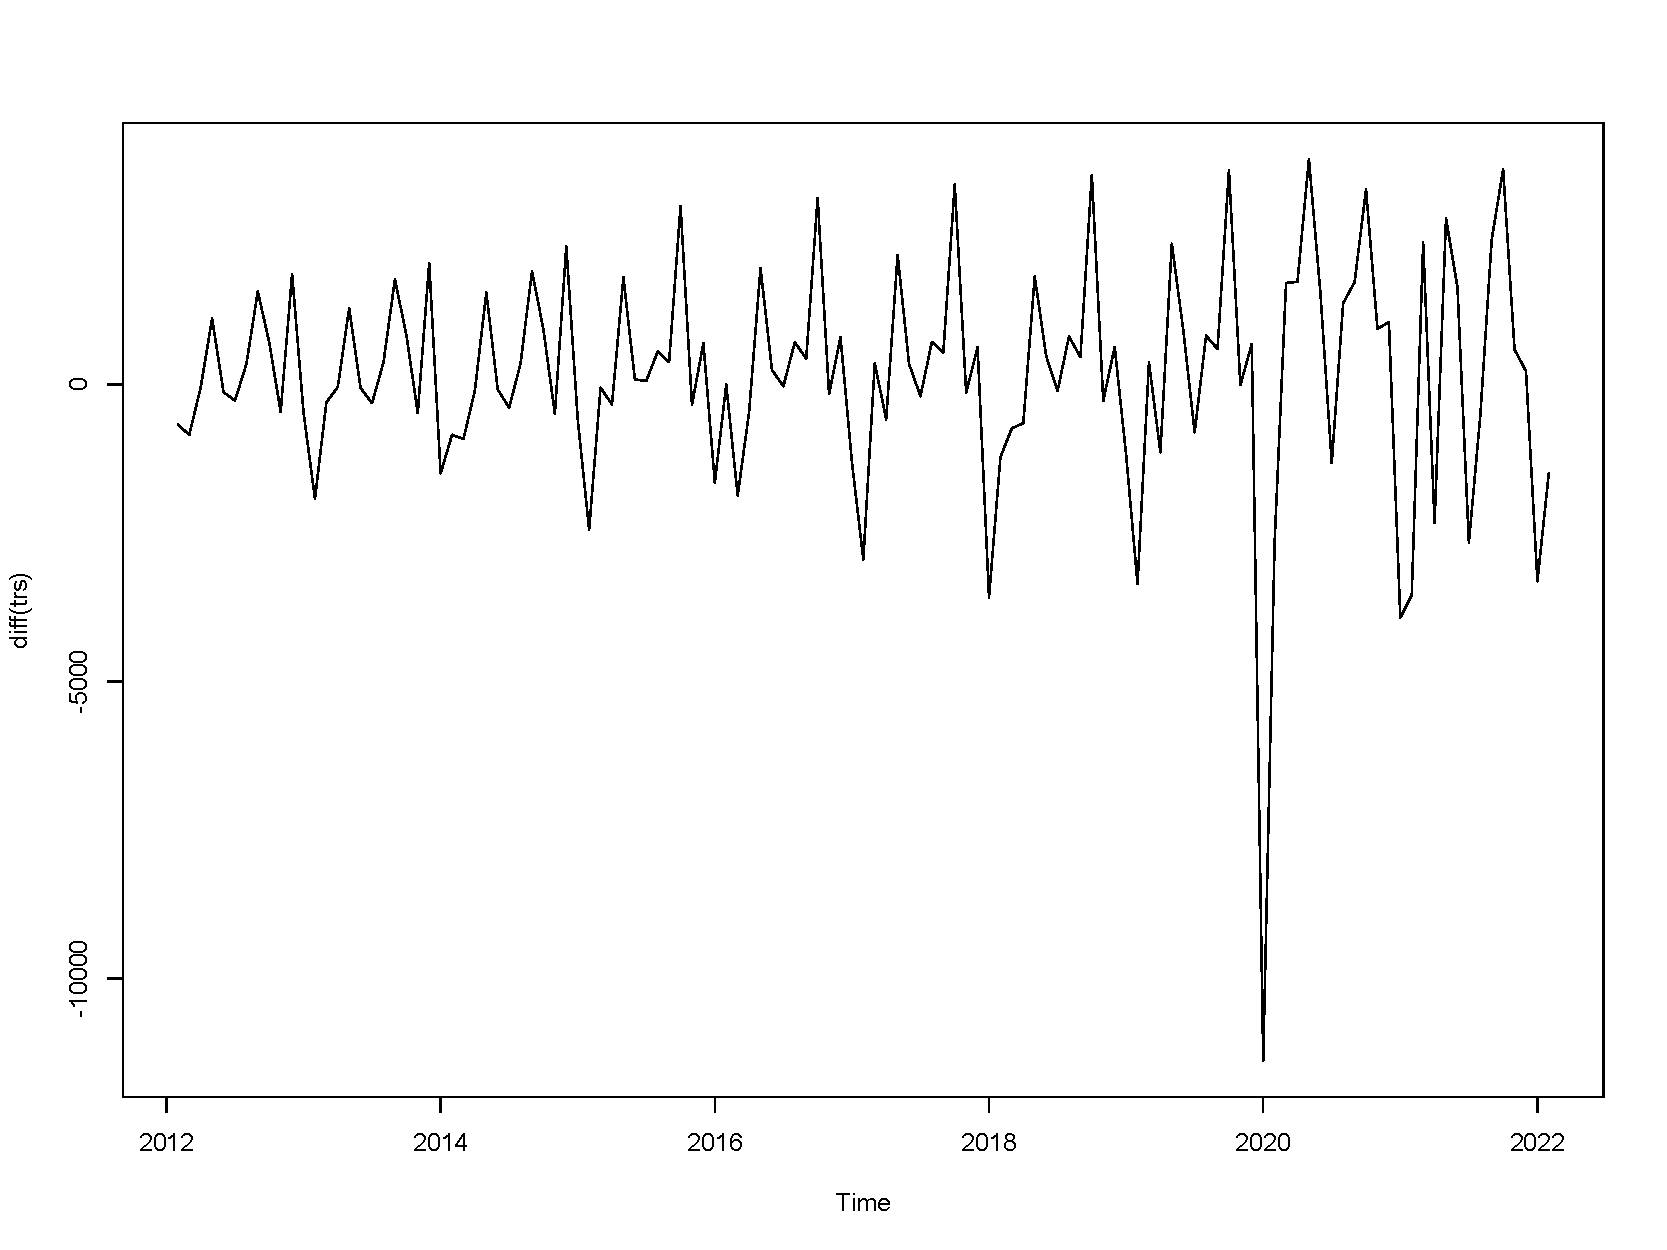
\includegraphics[width=0.7\textwidth]{diff_TRS.pdf} %插入图片,[]中设置图片大小,{}中是图片文件名
  \caption{对原序列做一阶差分后} %最终文档中希望显示的图片标题
  \label{diff_TRS} %用于文内引用的标签
\end{figure} 

在对差分后的序列做\(ADF\)检验:
\begin{table}[H]
  \centering
  \caption{\(ADF\)检验}
    \begin{tabular}{l|r}
    \multicolumn{2}{c}{ Augmented Dickey-Fuller Test} \\
    \hline
    Lag Order: & 1 \\
    Dickey-Fuller: & -7.5267\\
    P Value  & 0.01 \\
    \end{tabular}%
  \label{tab:ADF_diff}%
\end{table}%

由于\(p<0.05\)所以拒绝原假设,差分后的序列是平稳的,
即通过一阶差分去掉了原序列线性的趋势因子。

\subsubsection*{随机性检验}
尽管\(\hat{X}_t\)为平稳序列,但是如白噪声等纯随机序列
也是平稳序列,若\(\hat{X}_t\)是纯随机序列,则没有建模研究价值
价值,于是采用\(Ljung-Box\)检验随机性

假设\(H_0:\rho _1 = \rho _2 = \cdots = \rho _n = 0\)
则对所有的\(k>0\),样本的自相关系数服从:
\begin{equation}
  \hat{\rho}_k \approx N(0,\frac{1}{n})
\end{equation}

其中\(n\)为样本量,通过检验统计量:
\begin{equation}
  Q_{LB}(m) = n (n+2)\sum_{k=1}^{m}{\frac{\hat{\rho_{k}}^2}{n-k}} ~\chi^2(m)
\end{equation}

得到的\(Ljung-Box\)检验结果为:
% Table generated by Excel2LaTeX from sheet 'Sheet1'
\begin{table}[H]
  \centering
  \caption{\(Ljung-Box\)检验}
    \begin{tabular}{l|r}
    \multicolumn{2}{c}{Ljung-Box test} \\
    \hline
    X-squared  & \multicolumn{1}{r}{494.39} \\
    df    & \multicolumn{1}{r}{6} \\
    p-value & < 2.2e-16 \\
    \end{tabular}%
  \label{tab:Ljung-Box}%H
\end{table}%

由于\(p<0.05\)所以拒绝原假设,则\(\hat{X}_t\)为非随机序列,可进行下一步建模。


\subsection{无季节性的ARIMA模型建立}
给定一个差分\(d\)阶的时间序列\(y_t\),\(ARIMA(p,d,q)\)模型如下:
\begin{equation}
  y_t=c+\sum_{i=1}^p{\phi_i y_{t-i}}+\sum_{i=1}^q{\theta_i\varepsilon_{t-i}}+\varepsilon_t
\end{equation}

或者写为\cite{Rob} \[(1-\phi_1B - \cdots - \phi_p B^p)  (1-B)^d y_{t} = c + (1 + \theta_1 B + \cdots + \theta_q B^q)\varepsilon_t\]

其中\(\varepsilon_t\)是白噪声序列, \(p\)是自回归的阶数,\(q\)是移动平均的阶数。

平稳序列的自相关函数\(ACF\)与时间间隔\(k\)有关,并通过\(ACF\)相关系数决定\(q\):
\begin{equation}
  \rho_h = \rho(y_t,y_{t+k}) =\frac{Cov(y_t,y_{t+k})}{\sigma_t \sigma_{t+k}}
\end{equation}

\(ACF\)图显示了\(y_t\)与\(y_{t-k}\)之间相关性,但是滞后阶数\(1,2,\cdots,k-1\)之间存在依赖
关系\cite{Rob},例如若\(y_t\)与\(y_{t-1}\)自相关,那么\(y_t\)与\(y_{t-2}\)一定自相关,
因为他们都通过与\(y_{t-1}\)直接相关,而间接相关,为了分离\(y_{t-1},
y_{t-2},\cdots,y_{t-k+1}\)的干扰,直接得到\(y_t\)与\(y_{t-k}\)之间的相关性,通过\(PACF\)估计\(P\)值,由于历史白噪声\(\varepsilon_{t-k}\)通过影响历史观测值来间接影响
当前\(y_t\)所以用\(ACF\)估计\(q\)值,绘出一阶差分后\(\hat{X}_t\)的\(ACF\)和\(PACF\)图(临界值\(\frac{\pm1.96}{T}\)以用虚线标出):
\begin{figure}[H] %H为当前位置,!htb为忽略美学标准,htbp为浮动图形
  \centering %图片居中
  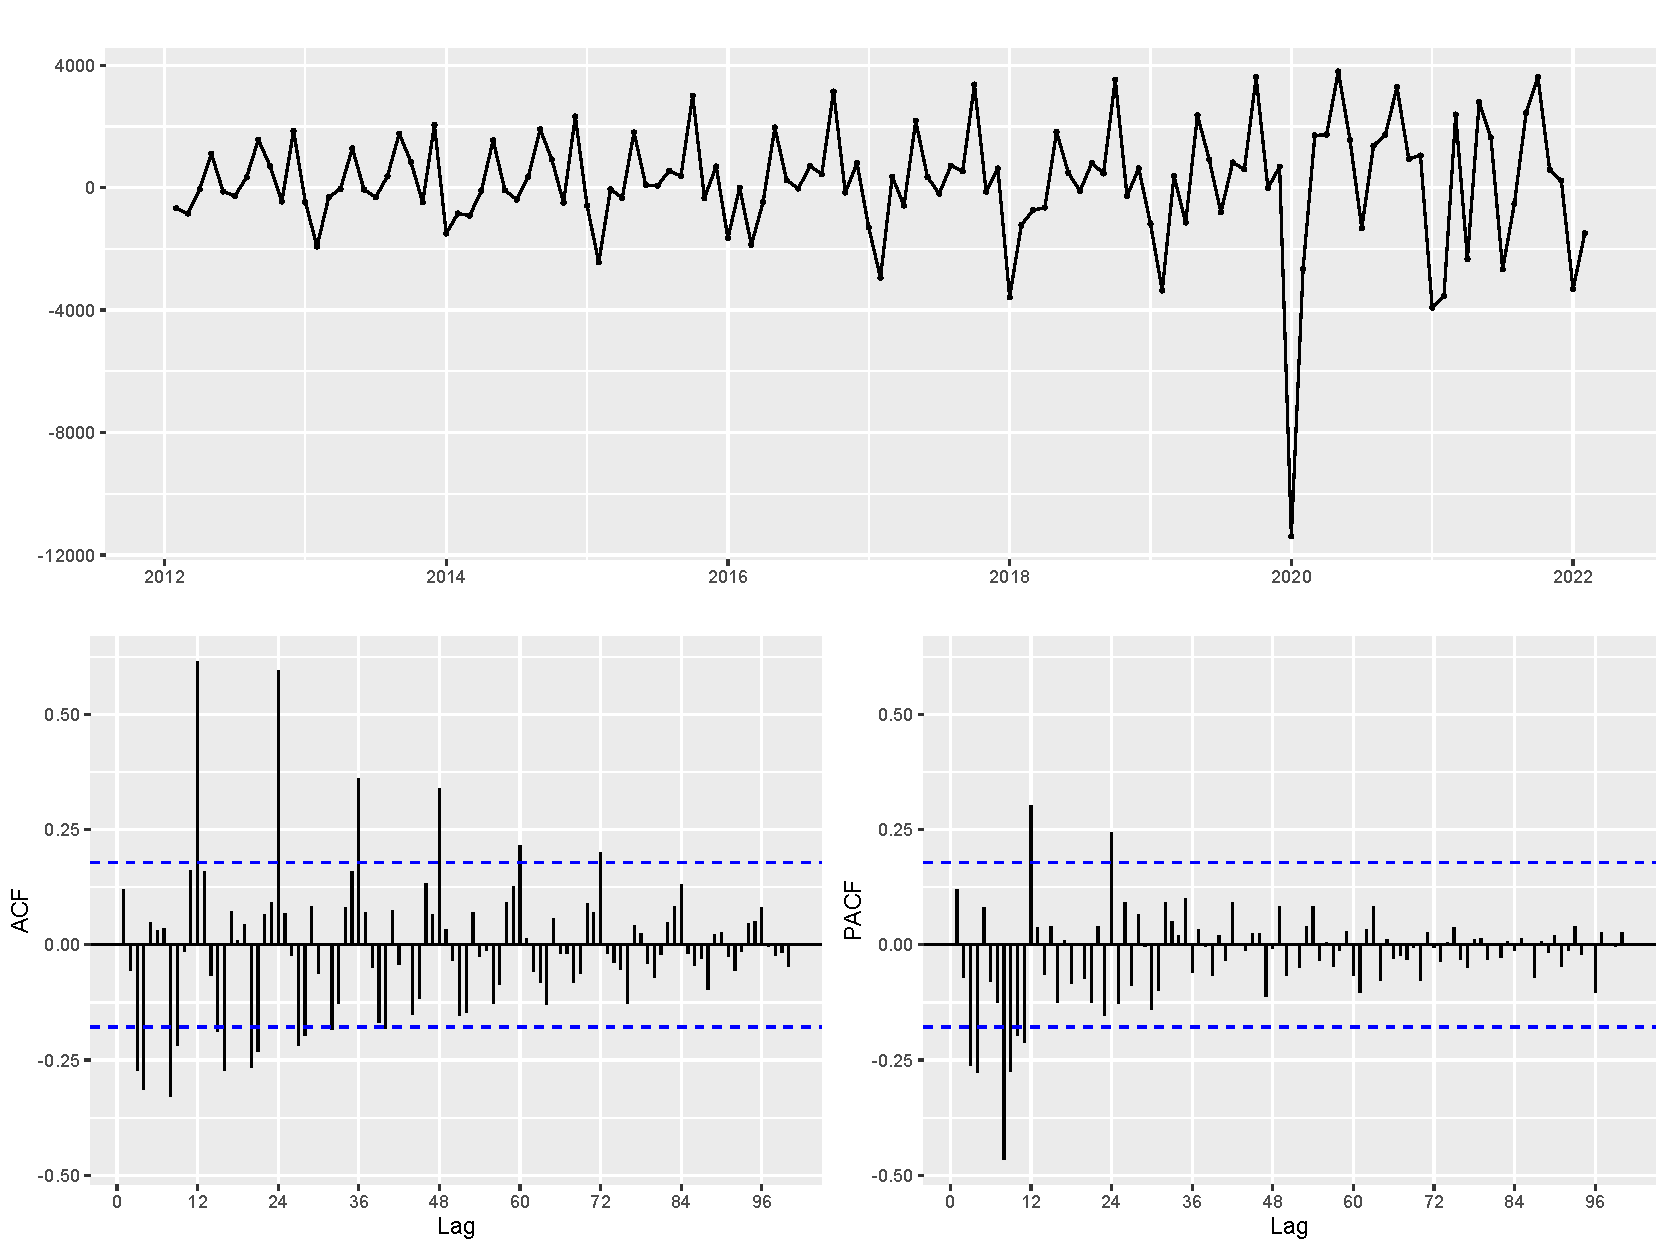
\includegraphics[width=1\textwidth]{acf_pacf.pdf} %插入图片,[]中设置图片大小,{}中是图片文件名
  \caption{ACF 和 PACF} %最终文档中希望显示的图片标题
  \label{acf_pacf} %用于文内引用的标签
  \end{figure} 
  \subsection{季节性的ARIMA模型}
  通过图\ref{acf_pacf}发现在滞后阶数\(lag\)值很高时才出现拖尾,会导致参数过多发生
  过拟合现象, 而且通过图\ref{decompose}得到消费总额应该是呈现明显季节波动
  所以考虑将一阶差分序列\(\hat{X}_t\)分解为季节部分和剩下的非季节部分\cite{Rob}:
\begin{center}
  ARIMA\;\;\;\;	\((p, d, q)\)	\;\;\;\;\; \((P, D, Q)_{m}\) \label{Season_decompose}
\end{center}

其中\(m=12\)为观测周期,可以将模型写成季节
部分与非季节部分的乘积,例如对于\(ARIMA(1,1,1)(1,1,1)_m\)
模型:
\begin{equation}
  (1 - \phi_{1}B)~(1 - \Phi_{1}B^{12})~(1 - B)~(1 - B^{4})y_{t} = (1 + \theta_{1}B)~ (1 + \Theta_{1}B^{4})\varepsilon_{t}
\end{equation}

 \subsection{参数估计}
 为先消除季节型波动,对一阶差分后\(\hat{X}_t\)做季节性差分,得到
 \(X'_{t}\) = \(\hat{X}_t-\hat{X}_{t-12}\),绘出相关图像:
 \begin{figure}[H] %H为当前位置,!htb为忽略美学标准,htbp为浮动图形
  \centering %图片居中
  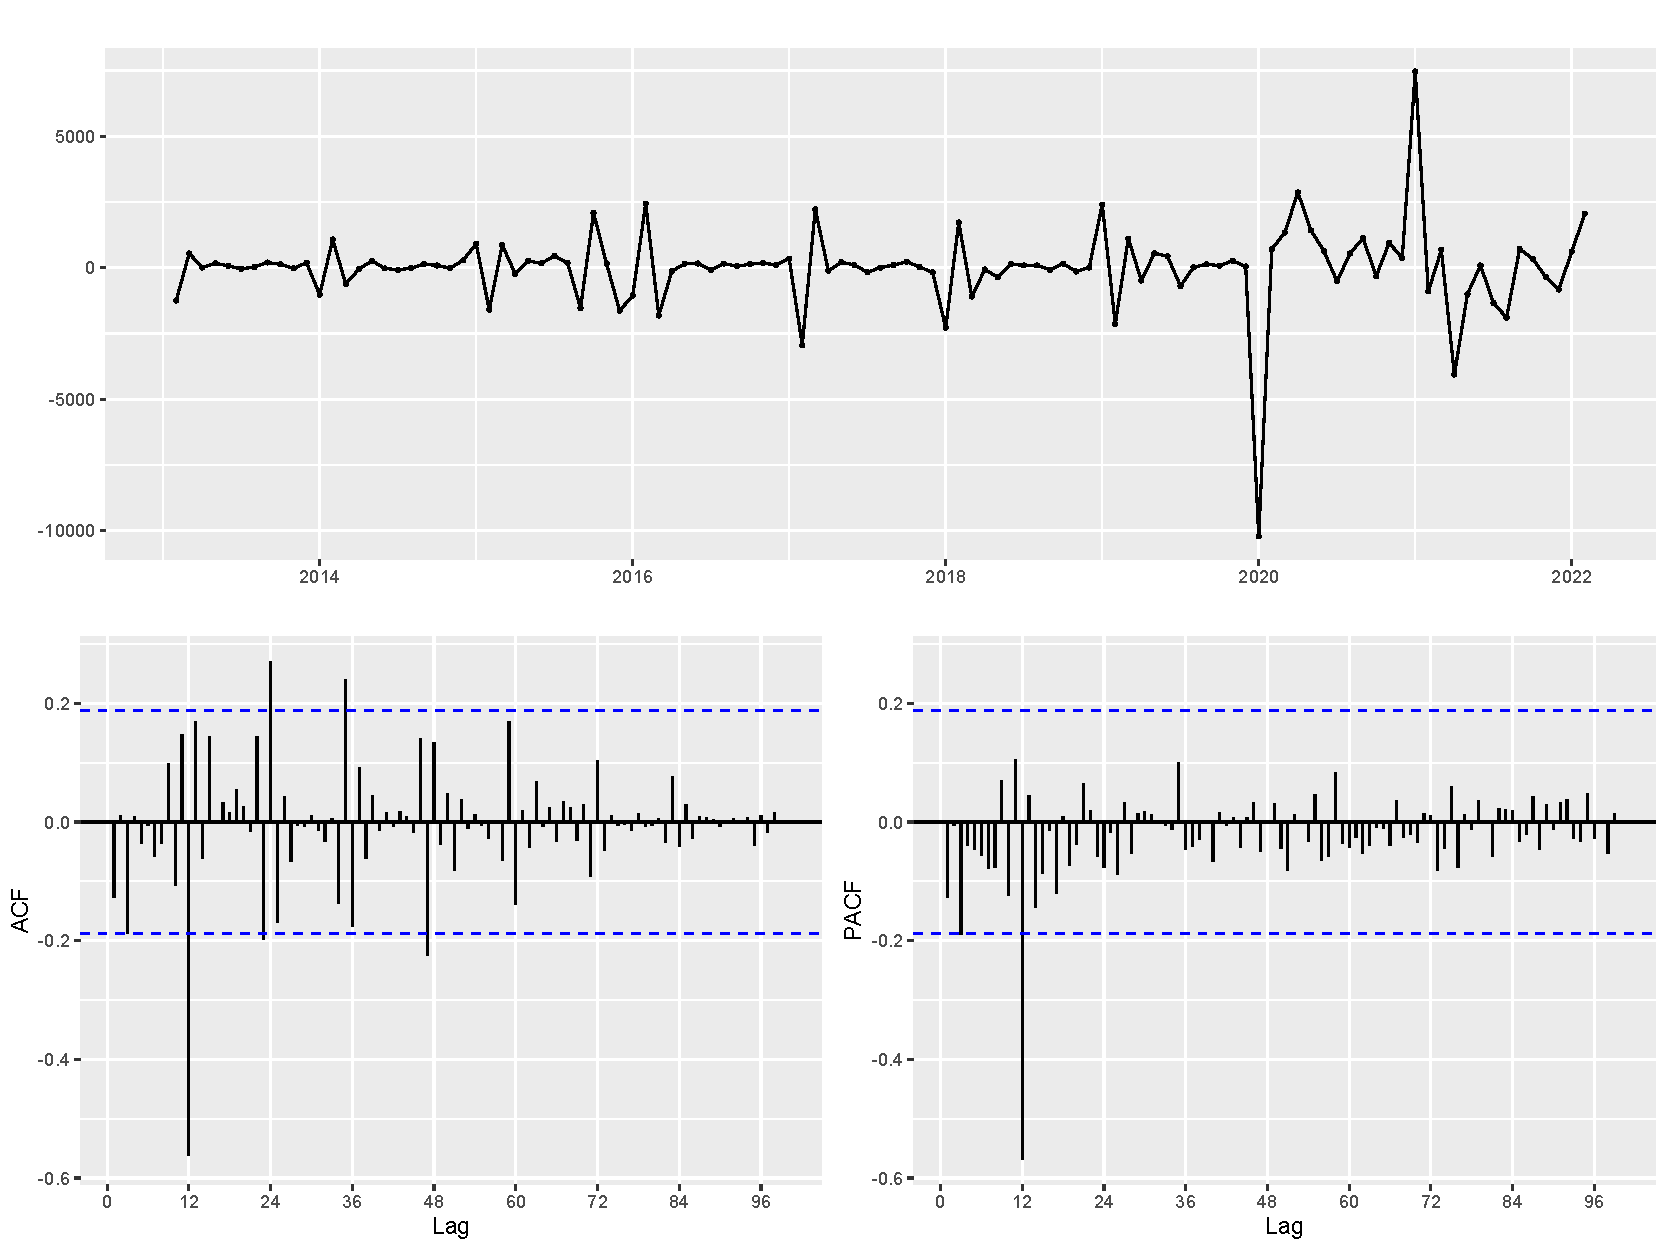
\includegraphics[width=1\textwidth]{Season_diff.pdf} %插入图片,[]中设置图片大小,{}中是图片文件名
  \caption{季节差分后 ACF 和 PACF} %最终文档中希望显示的图片标题
  \label{season_diff} %用于文内引用的标签
  \end{figure}
  \subsection{模型的选择}
  从相关系数图看出相比于图\ref{acf_pacf}, 相关系数的的衰减速度
  加快很多,对于季节部分的ACF和PACF图(即\(Lag=12n\),n对应季节部分的滞后系数)
  ,都在lag=12后产生拖尾。因此可确定\ref{Season_decompose}中的季节部分相应系数\(P=1 , Q=1\)

  但对于非季节部分的ACF和PACF图较难判断在何种滞后系数后产生拖尾,因此利用AIC,AICc,BIC准则定量的确定在何种
  系数下的模型最优:
  \begin{equation*}
    \text{AIC} = -2log(L) + 2(p+q+k+1)
  \end{equation*}
  其中\(L\)是似然数据的似然函数,最后一项为参数个数(包含了余项的方差)\(k=0\)若\(c=0\),\(k=1\)若\(c\neq0\)
  对于ARIMA模型而言,修正过的AIC值可以被表示为\cite{Rob}:
  \begin{equation*}
    \text{AICc} = \text{AIC} + \frac{2(p+q+k+1)(p+q+k+2)}{T-p-q-k-2}
  \end{equation*}

  并且贝叶斯信息准则(BIC)如下:\[\text{BIC} = \text{AIC} + [\log(T)-2](p+q+k+1)\]
  通过枚举p,q的值得到相应模型AIC,AICc,BIC如下:
% Table generated by Excel2LaTeX from sheet 'Sheet1'
\begin{table}[htbp]
  \centering
  \caption{Add caption}
    \begin{tabular}{c|ccc}
    相应的ARIMA模型 & AIC   & AICc  & BIC \\
    \hline
    (0,1,0)(1,1,1)[12] & 1876.32 & 1876.55 & 1884.4 \\
    (0,1,1)(1,1,1)[12] & 1878.32 & 1878.7 & 1889.08 \\
    (0,1,2)(1,1,1)[12] & 1877.96 & 1878.54 & 1891.41 \\
    (0,1,3)(1,1,1)[12]  & 1876.22 & 1877.04 & 1892.36 \\
    (1,1,1)(1,1,1)[12] & 1880.27 & 1880.86 & 1893.73 \\
    (1,1,2)(1,1,1)[12] & 1873.59 & 1874.41 & 1889.74 \\
    (1,1,3)(1,1,1)[12] & 1875.51 & 1876.62 & 1894.35 \\
    (2,1,1)(1,1,1)[12] & 1873.53 & 1874.36 & 1889.68 \\
    (2,1,2)(1,1,1)[12] & 1875.02 & 1876.13 & 1893.86 \\
    (3,1,0)(1,1,1)[12] & 1879.02 & 1879.84 & 1895.16 \\
    (3,1,1)(1,1,1)[12] & 1875.53 & 1876.64 & 1894.37 \\
    (3,1,2)(1,1,1)[12] & 1876.98 & 1878.79 & 1901.2 \\
    \end{tabular}%
  \label{choose optimal models}%
\end{table}%

  从表\ref{choose optimal models}中看出,\(ARIMA(2,1,1)(1,1,1)_{12}\)是最优的ARIMA模型。
  \subsection{残差检验}
  为说明残差纯随机变量,对残差\(\epsilon_t\)做Ljung-Box test检验:
  \begin{table}[H]
    \centering
    \caption{残差\(Ljung-Box\)检验结果}
      \begin{tabular}{l|l}
      \multicolumn{2}{c}{Ljung-Box test} \\
      \hline
      df    & \multicolumn{1}{r}{19} \\
      p-value & 0.90 \\
      \end{tabular}%
    \label{Ljung-Box of Residuals}%H
  \end{table}%
  \(p>0.05\)无法拒绝原假设,所得残差为白噪声序列,残差之间不存在自相关性。
  并且得到的残差图\ref{Redsiduals},残差基本符合正态分布要求:
  \begin{figure}[H] %H为当前位置,!htb为忽略美学标准,htbp为浮动图形
  \centering %图片居中
  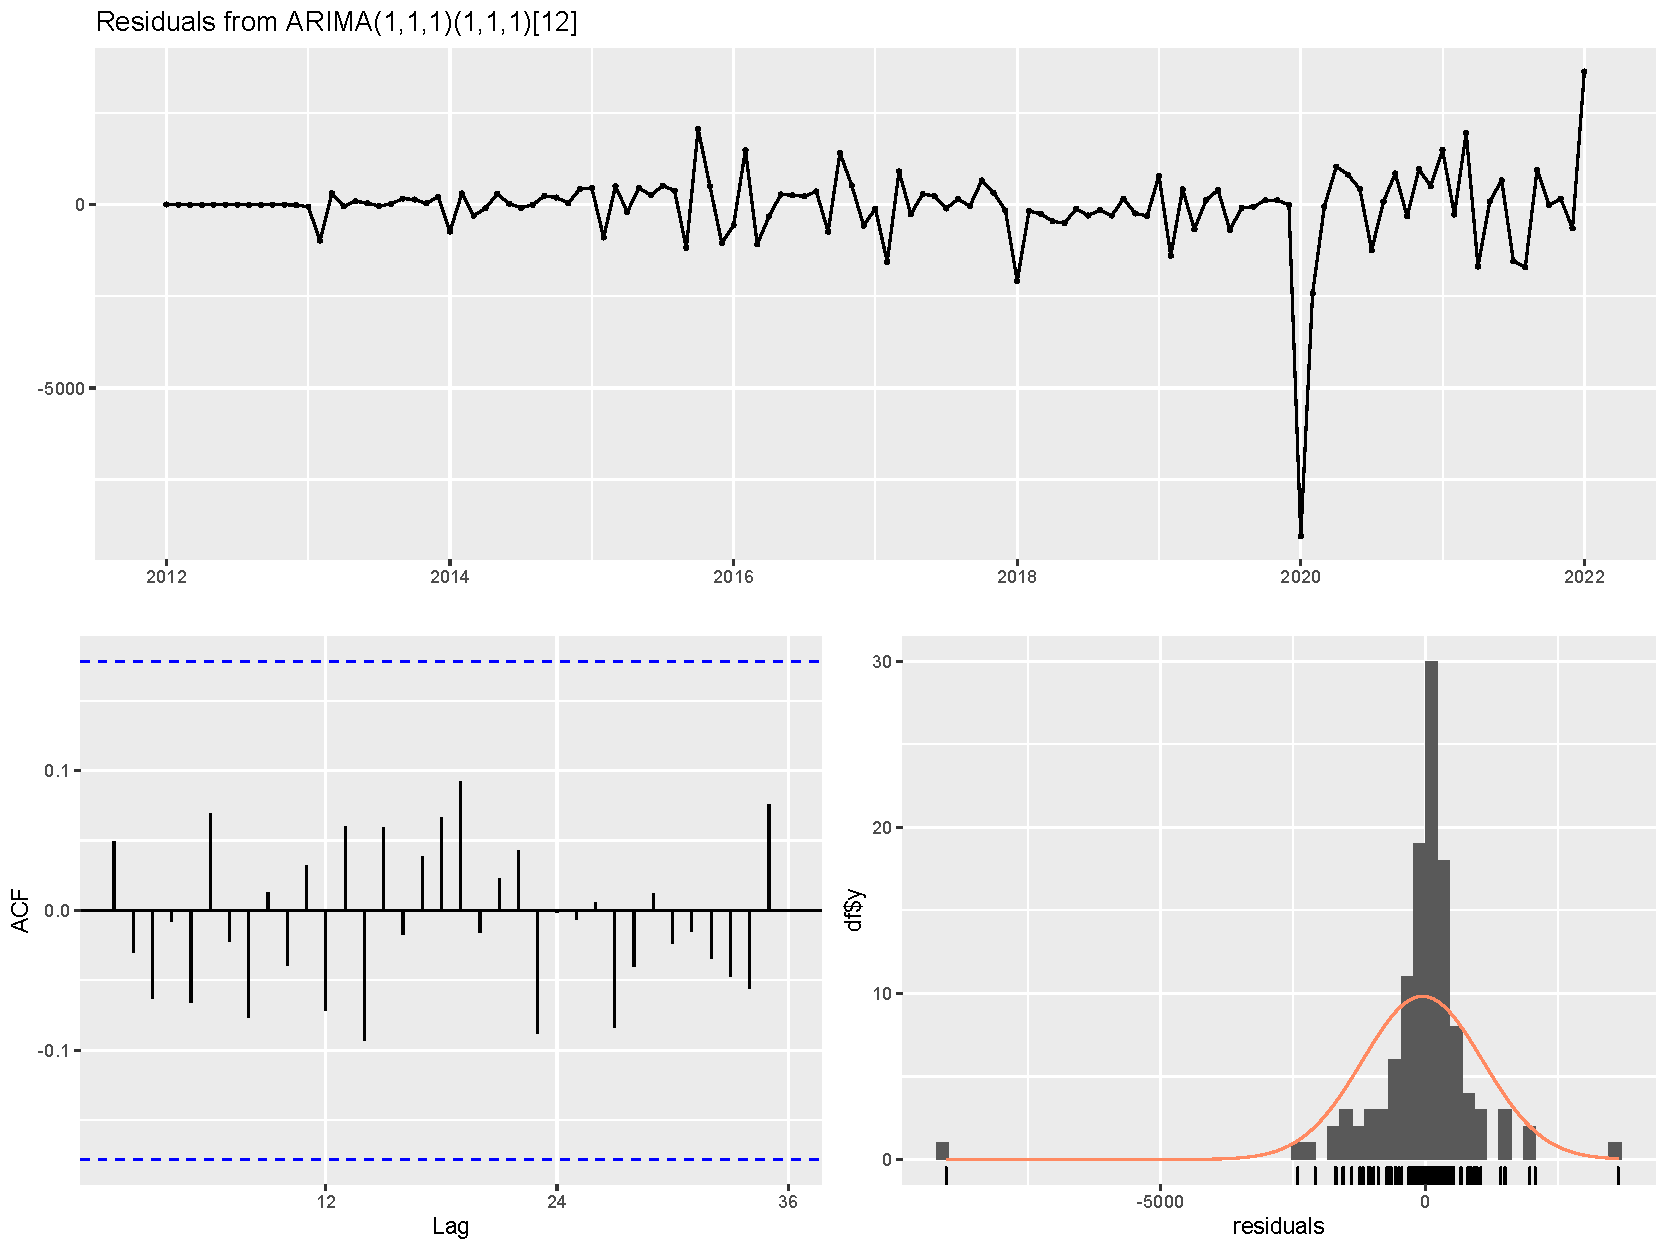
\includegraphics[width=0.8\textwidth]{Residuals.pdf} %插入图片,[]中设置图片大小,{}中是图片文件名
  \caption{\(ARIMA(2,1,1)(1,1,1)_{12}\)的残差图} %最终文档中希望显示的图片标题
  \label{Redsiduals} %用于文内引用的标签
  \end{figure} 
  为进一步说明,绘出正态Q-Q图\ref{Q-Qplot},所以残差符合正态分布要求:
  \begin{figure}[H] %H为当前位置,!htb为忽略美学标准,htbp为浮动图形
    \centering %图片居中
    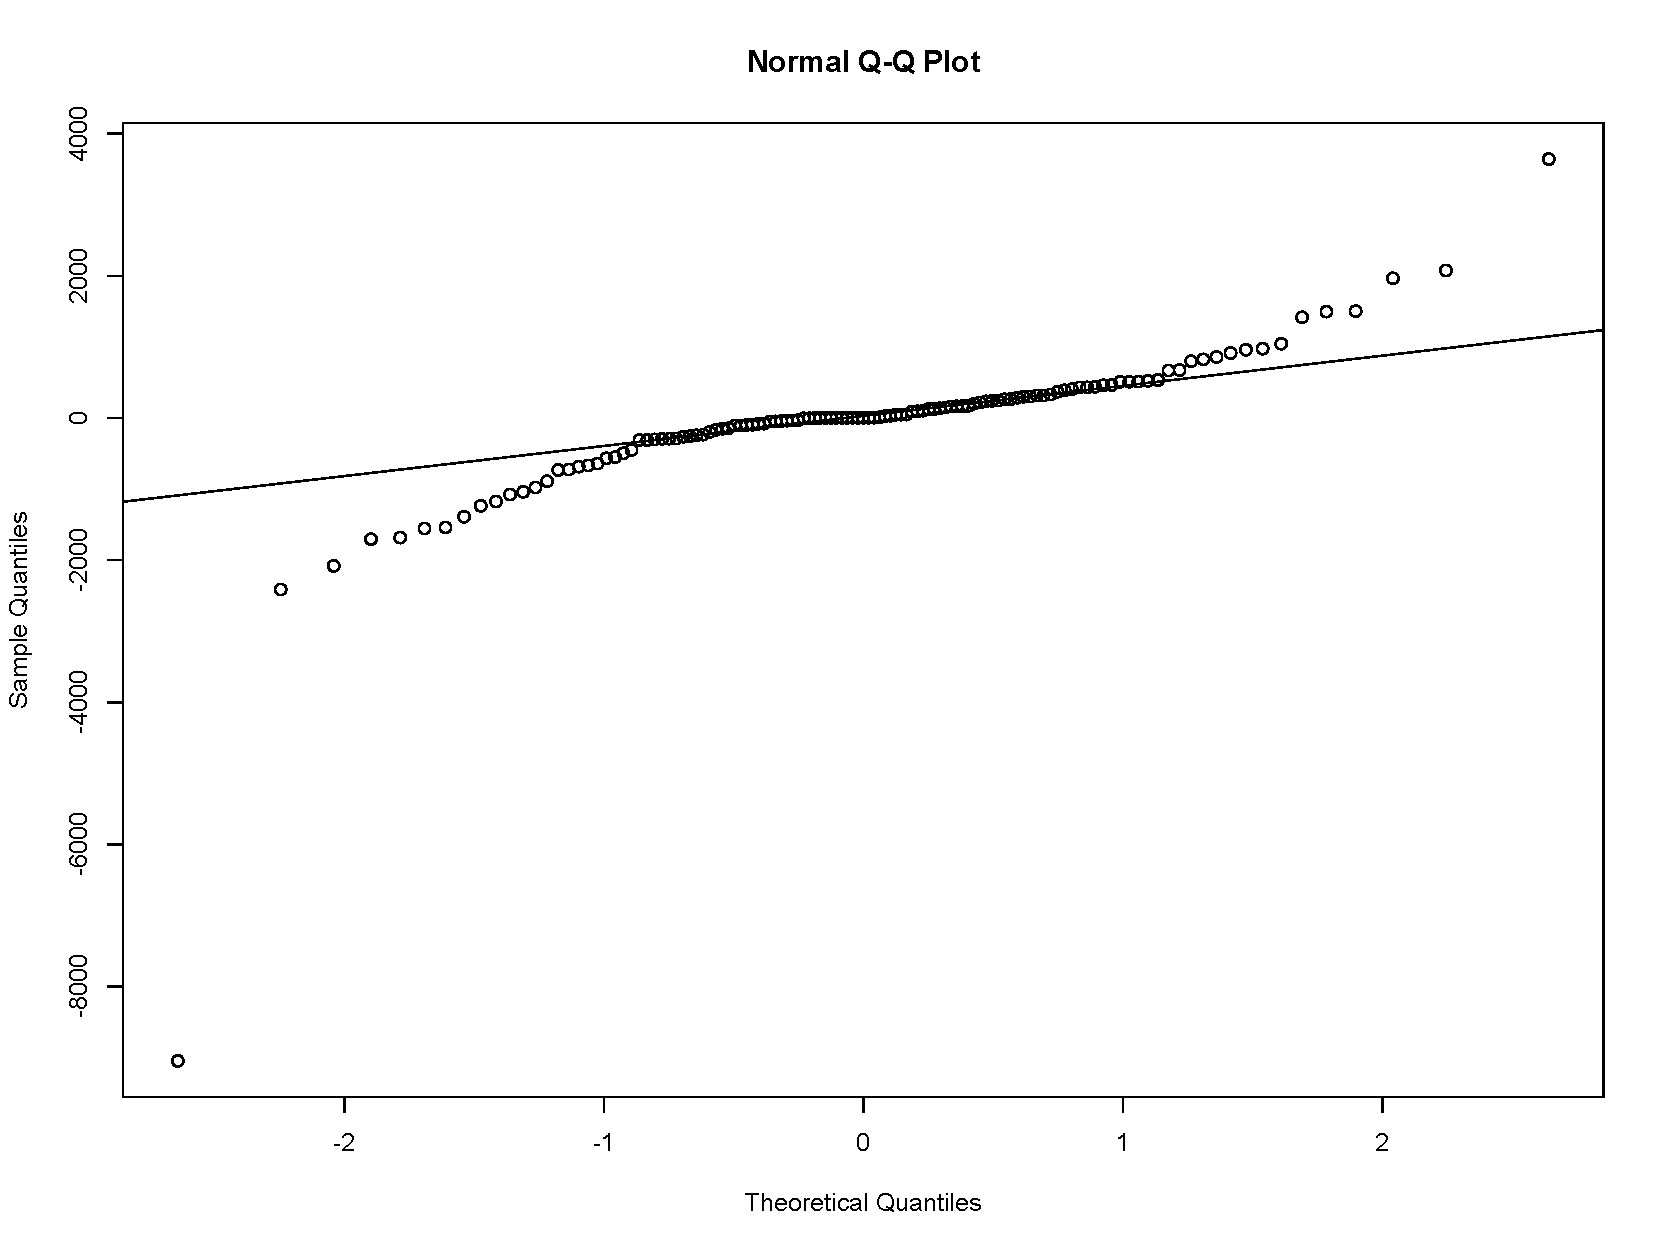
\includegraphics[width=0.8\textwidth]{Q-Qplot.pdf} %插入图片,[]中设置图片大小,{}中是图片文件名
    \caption{\(ARIMA(2,1,1)(1,1,1)_{12}\)的残差Q-Q图} %最终文档中希望显示的图片标题
    \label{Q-Qplot} %用于文内引用的标签
  \end{figure} 
  \subsection{未受疫情干预的预测}
  选取的训练集为表\ref{TRS}中2022年2月以前(包括二月).
  用得到的ARIMA模型对训练集进行拟合,以12个月划分序列。
  通过所有之前的数据拟合当前年份的数据(起始两年除外),拟合得到的12步拟合结果图\ref{traning_forecast}:
  \begin{figure}[H] %H为当前位置,!htb为忽略美学标准,htbp为浮动图形
    \centering %图片居中
    \begin{minipage}[t]{0.48\textwidth}
      \centering
      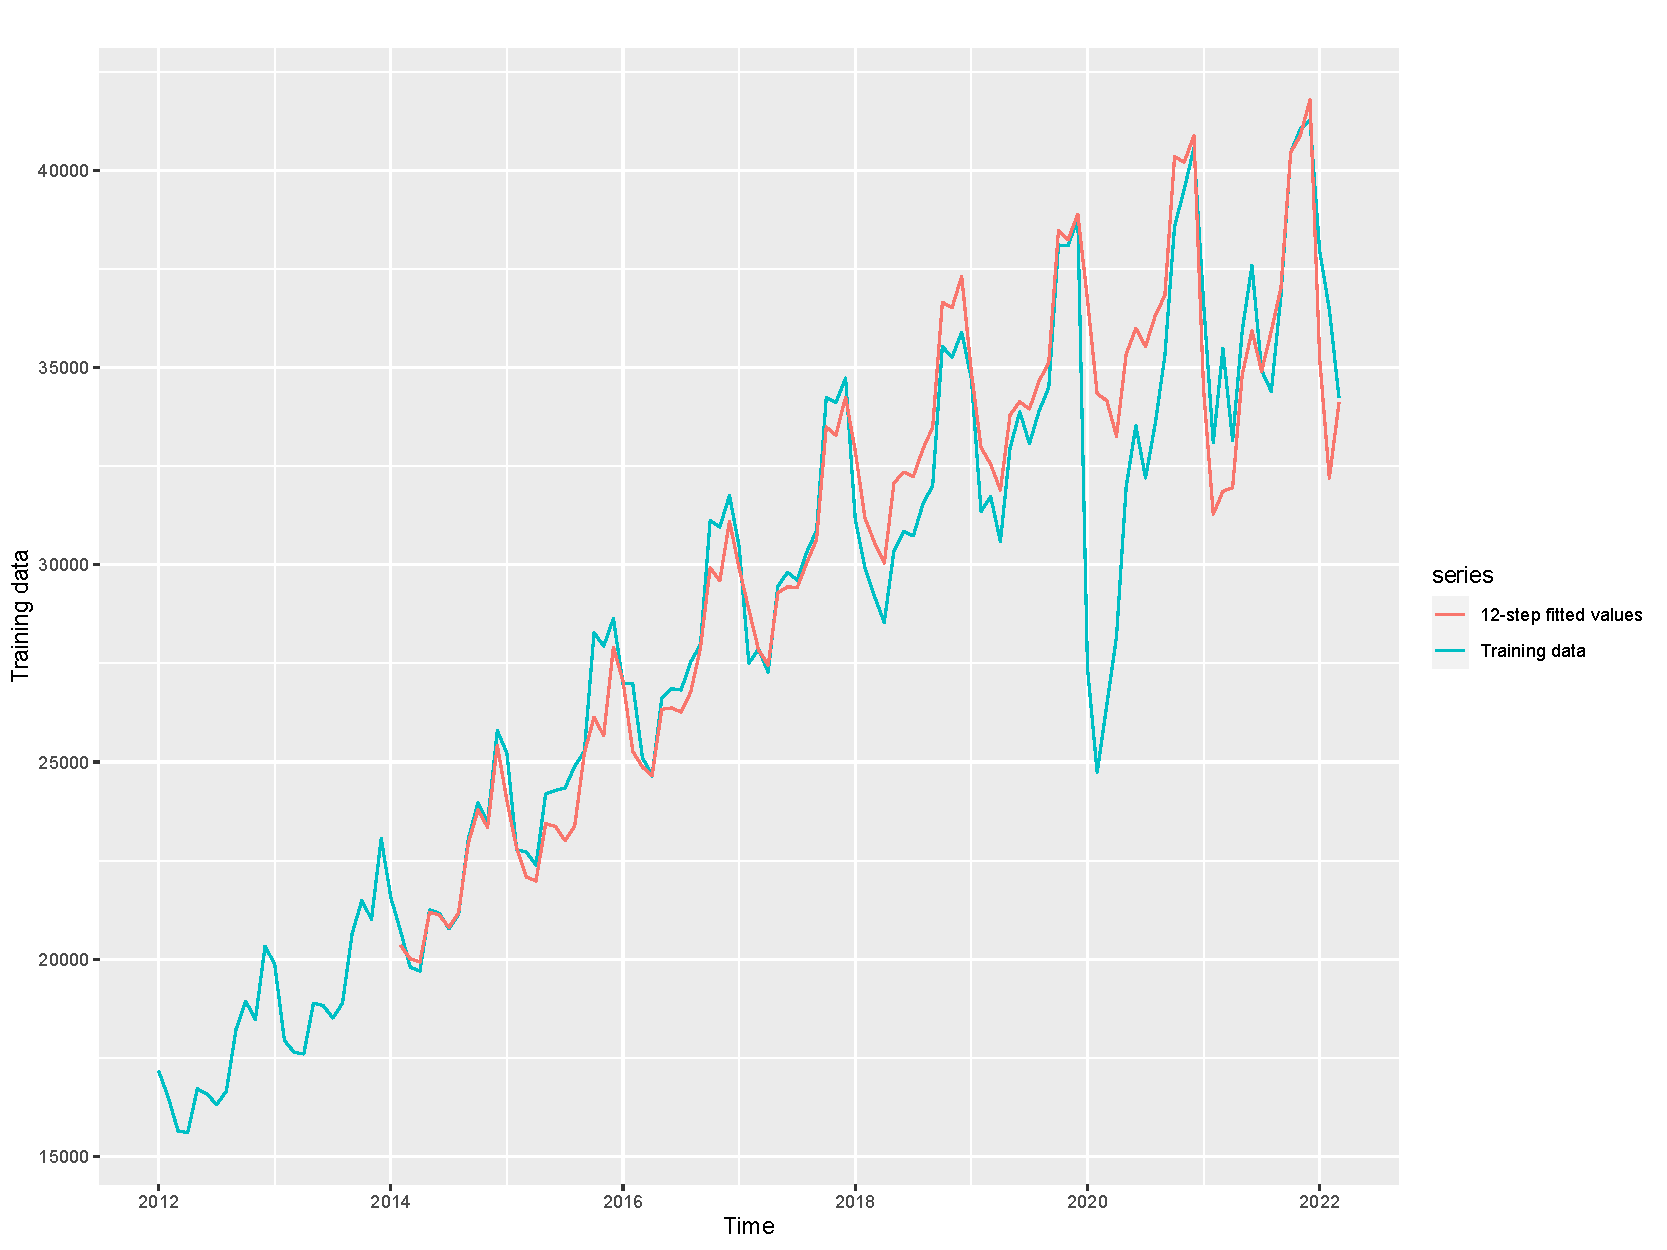
\includegraphics[width=1\textwidth]{training_forecast.pdf} %插入图片,[]中设置图片大小,{}中是图片文件名
      \caption{\small{\(ARIMA\)模型得到的12步拟合值}} %最终文档中希望显示的图片标题
      \label{traning_forecast} %用于文内引用的标签
    \end{minipage}
    \begin{minipage}[t]{0.48\textwidth}
      \centering %图片居中
      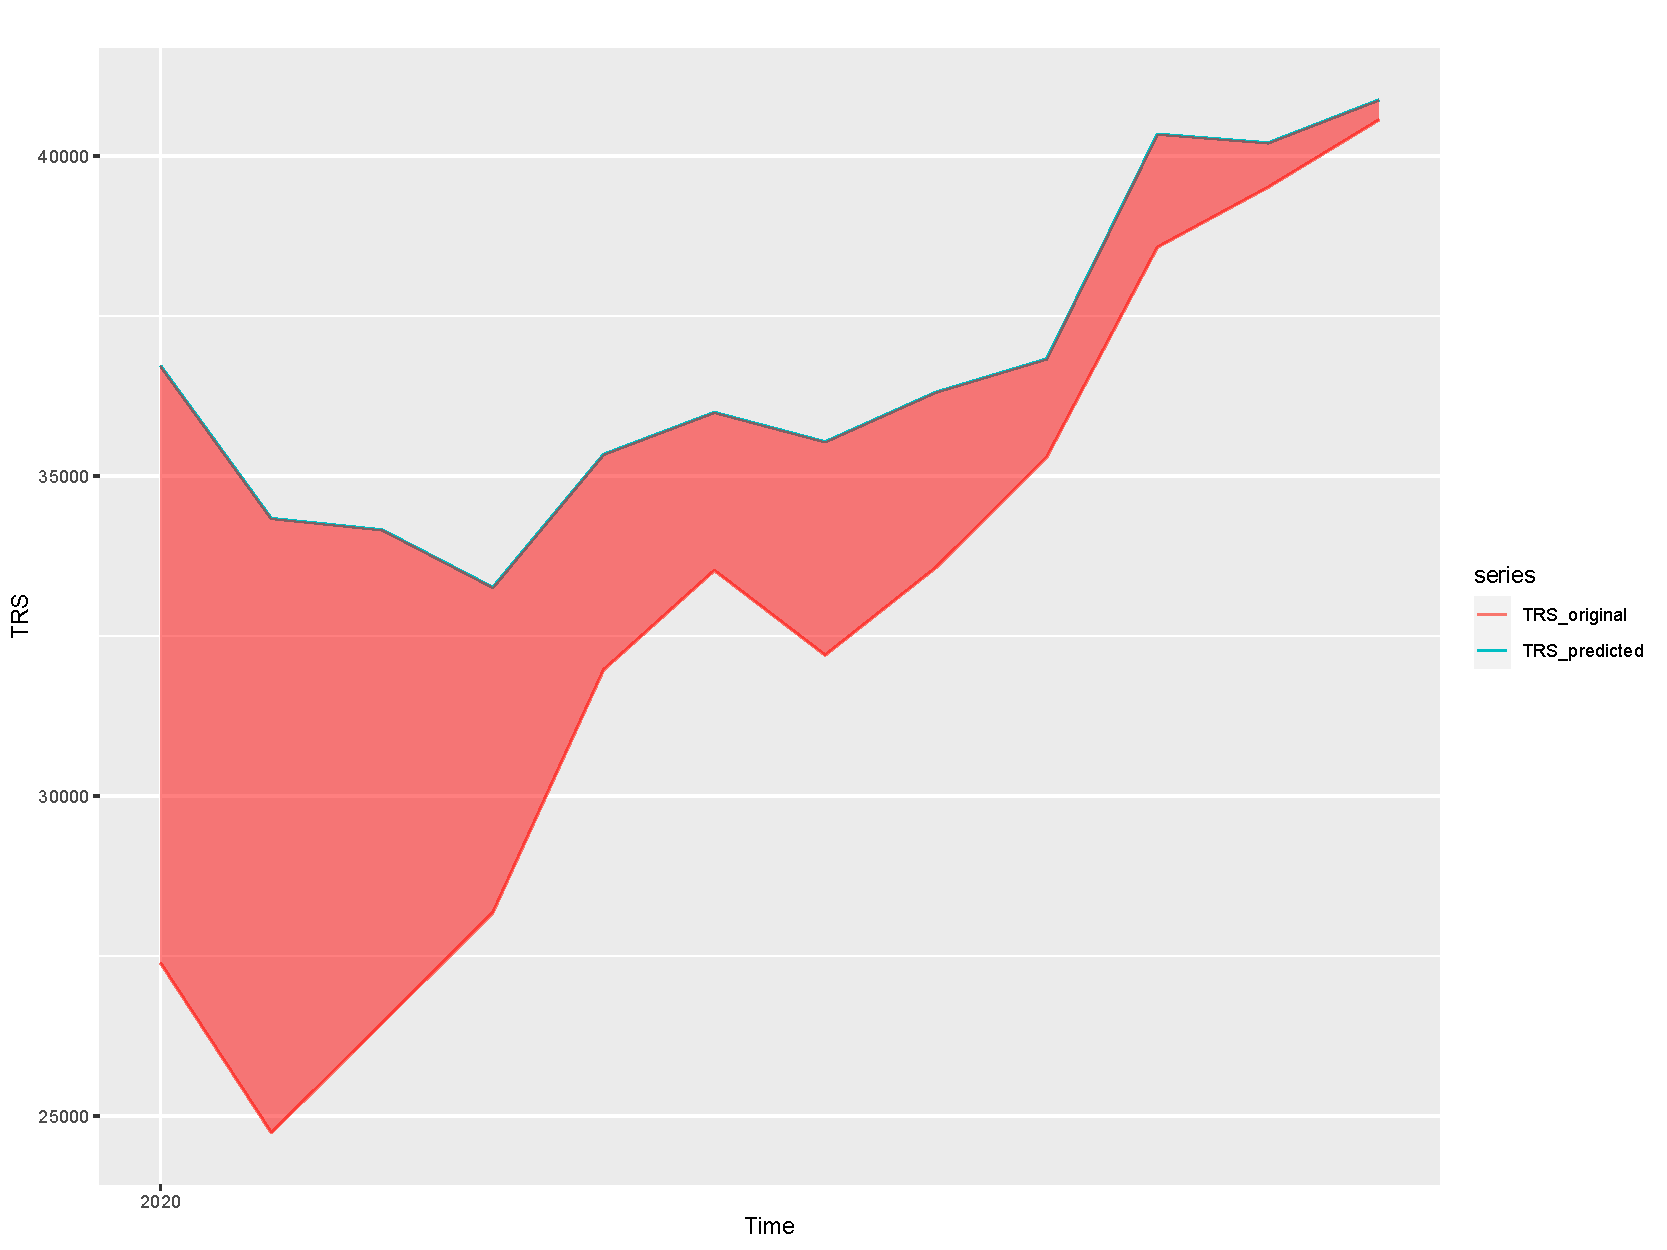
\includegraphics[width=1\textwidth]{trs_2020.pdf} %插入图片,[]中设置图片大小,{}中是图片文件名
      \caption{\small{2020年社会消费品零售总额的损失}} %最终文档中希望显示的图片标题
      \label{trs_2020} %用于文内引用的标签
    \end{minipage}
  \end{figure} 
  从图像上看,除去2020年初有所偏差外,其余部分都能较好拟合。由此也能从图中得出2020年
  疫情带来的社会消费品零售总额的损失为47934.05(亿元),为图\ref{trs_2020}中阴影部分。
  最终用此模型预测自2022年3月起10个月的预测结果如下,并给出\(80\% \text{和}95\%\)的置信区间。
  \begin{figure}[H] %H为当前位置,!htb为忽略美学标准,htbp为浮动图形
    \centering %图片居中
    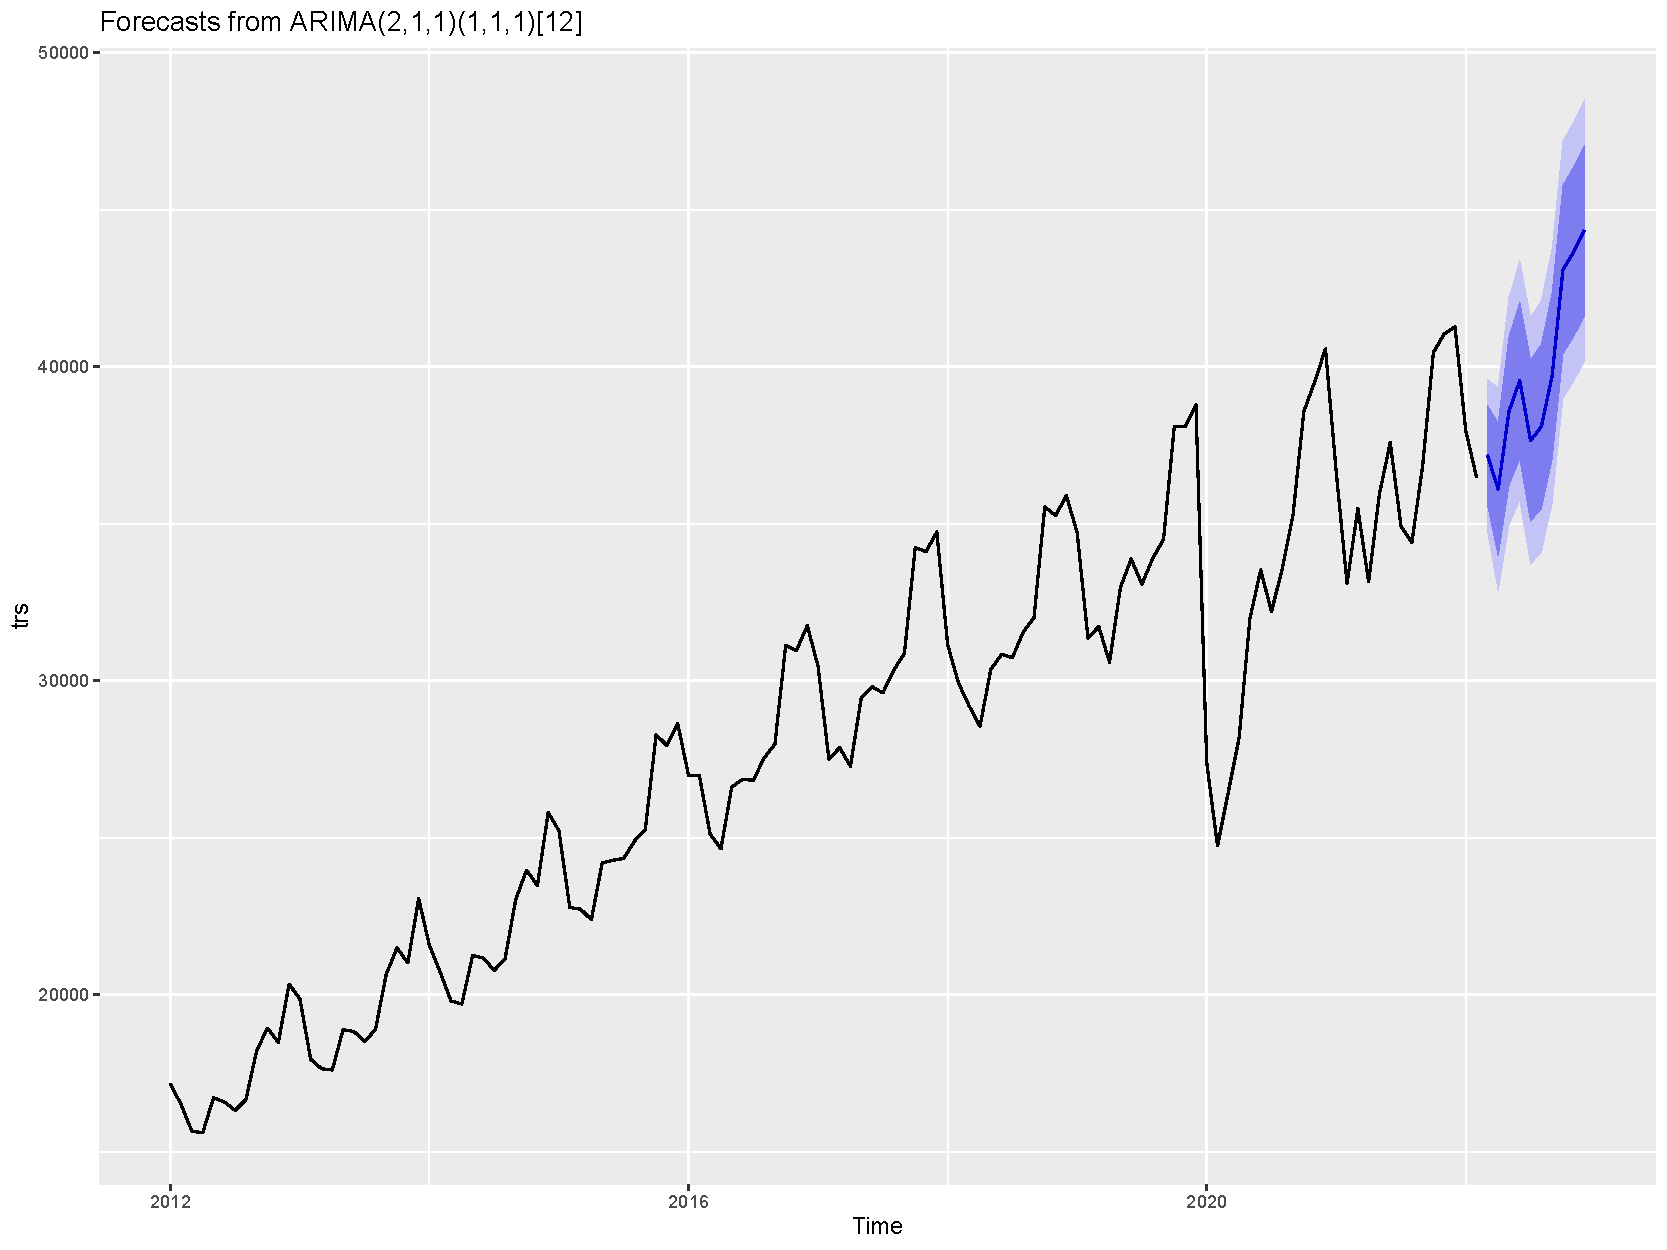
\includegraphics[width=0.7\textwidth]{forecast.pdf} %插入图片,[]中设置图片大小,{}中是图片文件名
    \caption{\(ARIMA(2,1,1)(1,1,1)_{12}\)模型对从3月起至2022年12月的预测值} %最终文档中希望显示的图片标题
    \label{forecast} %用于文内引用的标签
  \end{figure} 
  \section{干预分析模型的建立}
  \subsection{模型建立}
  假设疫情对经济的影响是突然开始,并且持续的,对持续性干预变量
  \[S_t^T = \begin{cases}
    0& \text{疫情发生前 t<T}\\
    1& \text{疫情发生后 t>=T}
  \end{cases}\]
  设\(\omega\)为干预未知的干预系数,\(Z_t\)为疫情发生后所产生的损失的时间序列,通过一阶差分获得平稳序列,
  则干预后的模型可写为
  \begin{equation}
      Z_t = \frac{\omega S_t^T}{\delta Z_{t-1}} \; 0<\delta<1
  \end{equation}
  经过变换,实际上为1阶自回归模型\cite{yandou}\[Z_t = \delta Z_{t-1} + \omega\]
  通过2020年的损失的社会消费品零售总额的数据\ref{trs_2020},
  将疫情对经济的冲击分为两个阶段,先是损失逐步扩大的过程,
  后是经济逐步恢复的时期。
  只考虑当损失逐渐恢复的一段,即从2020年2月至12月的损失。
  用最小二乘法的到参数的估计值,\(\delta =0.7328 , \omega =  72.1654 \)
  \subsection{残差检验}
  绘出回归拟合图像和残差图如下,  从残差分布曲线看,残差基本符合正态分布要求, 且通过Ljung-Box检验。:
  \begin{figure}[H] %H为当前位置,!htb为忽略美学标准,htbp为浮动图形
    \centering %图片居中
    \begin{minipage}[t]{0.48\textwidth}
      \centering
      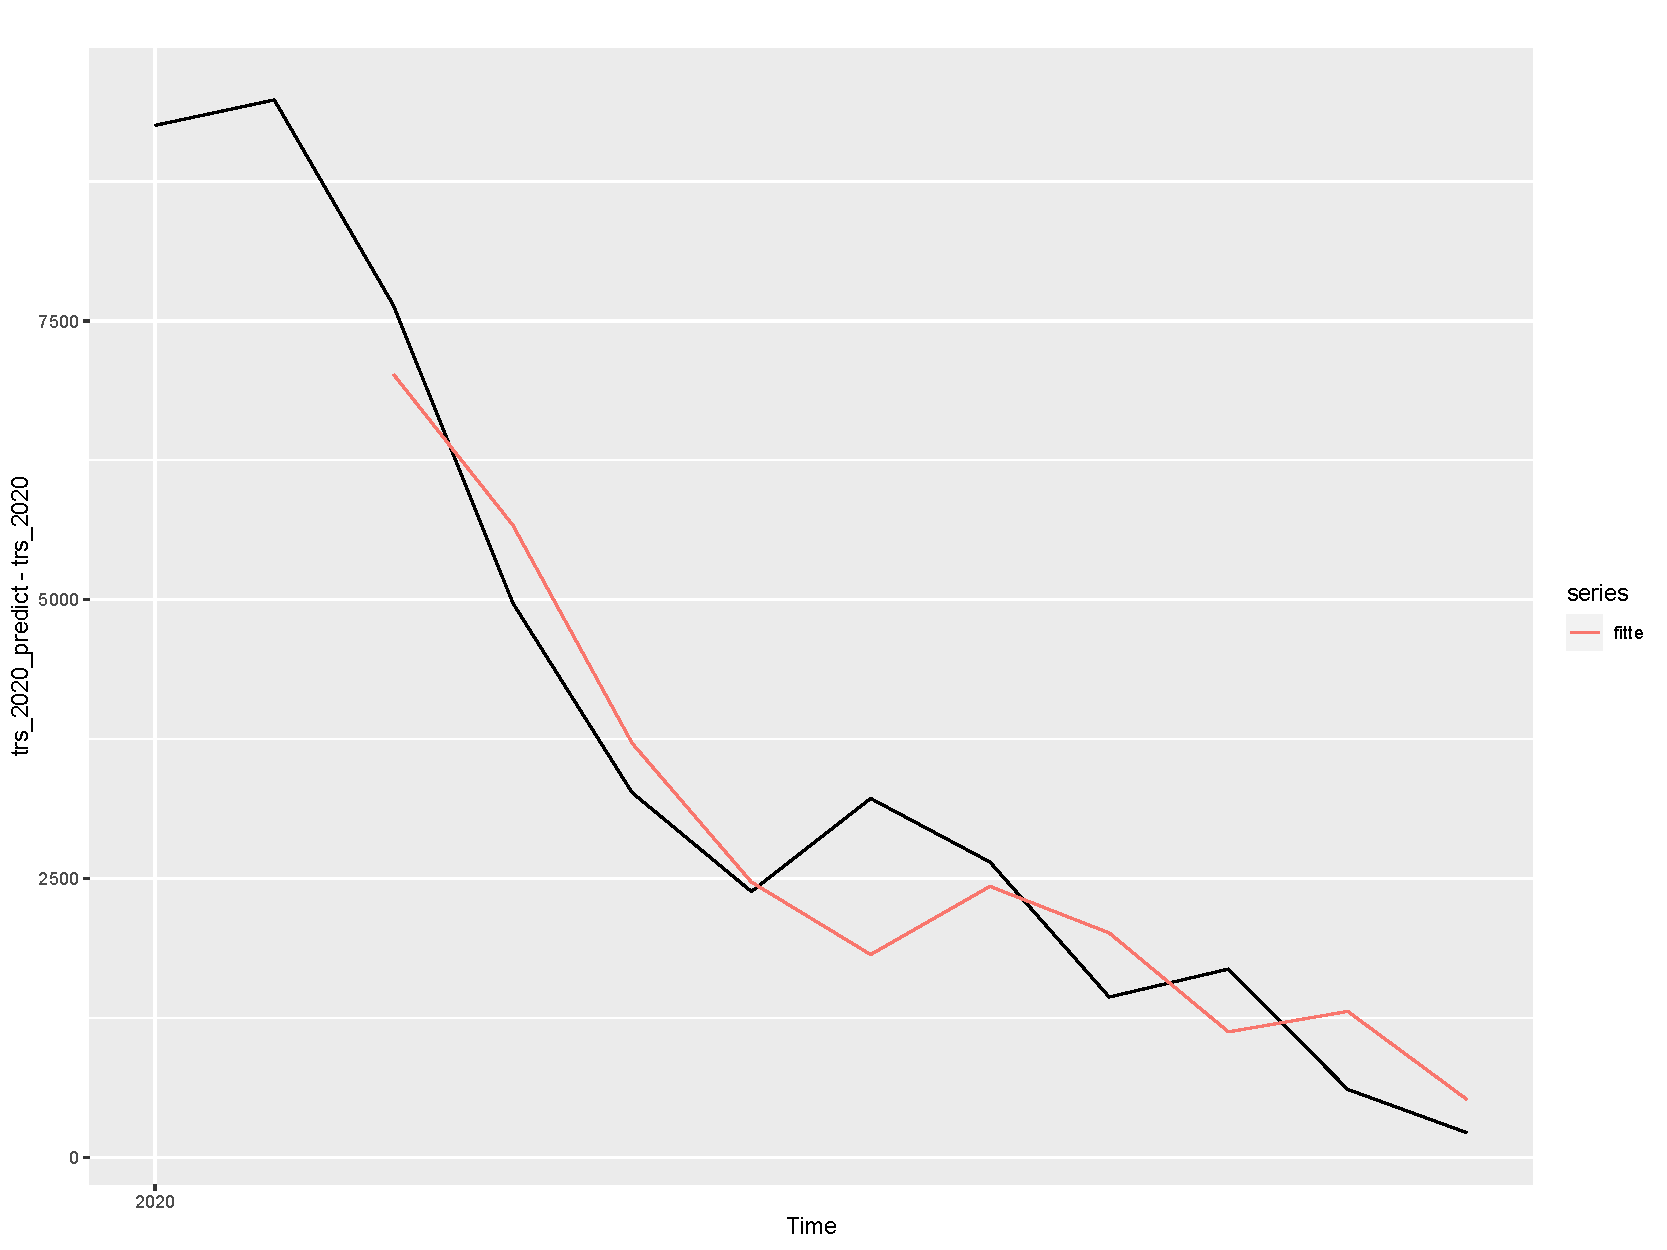
\includegraphics[width=1\textwidth]{fitted_loss_2020.pdf} %插入图片,[]中设置图片大小,{}中是图片文件名
      \caption{2020年社会消费品零售总额的损失图(红色为回归结果)} %最终文档中希望显示的图片标题
      \label{fitted_loss_2020} %用于文内引用的标签
    \end{minipage}
    \begin{minipage}[t]{0.48\textwidth}
      \centering %图片居中
      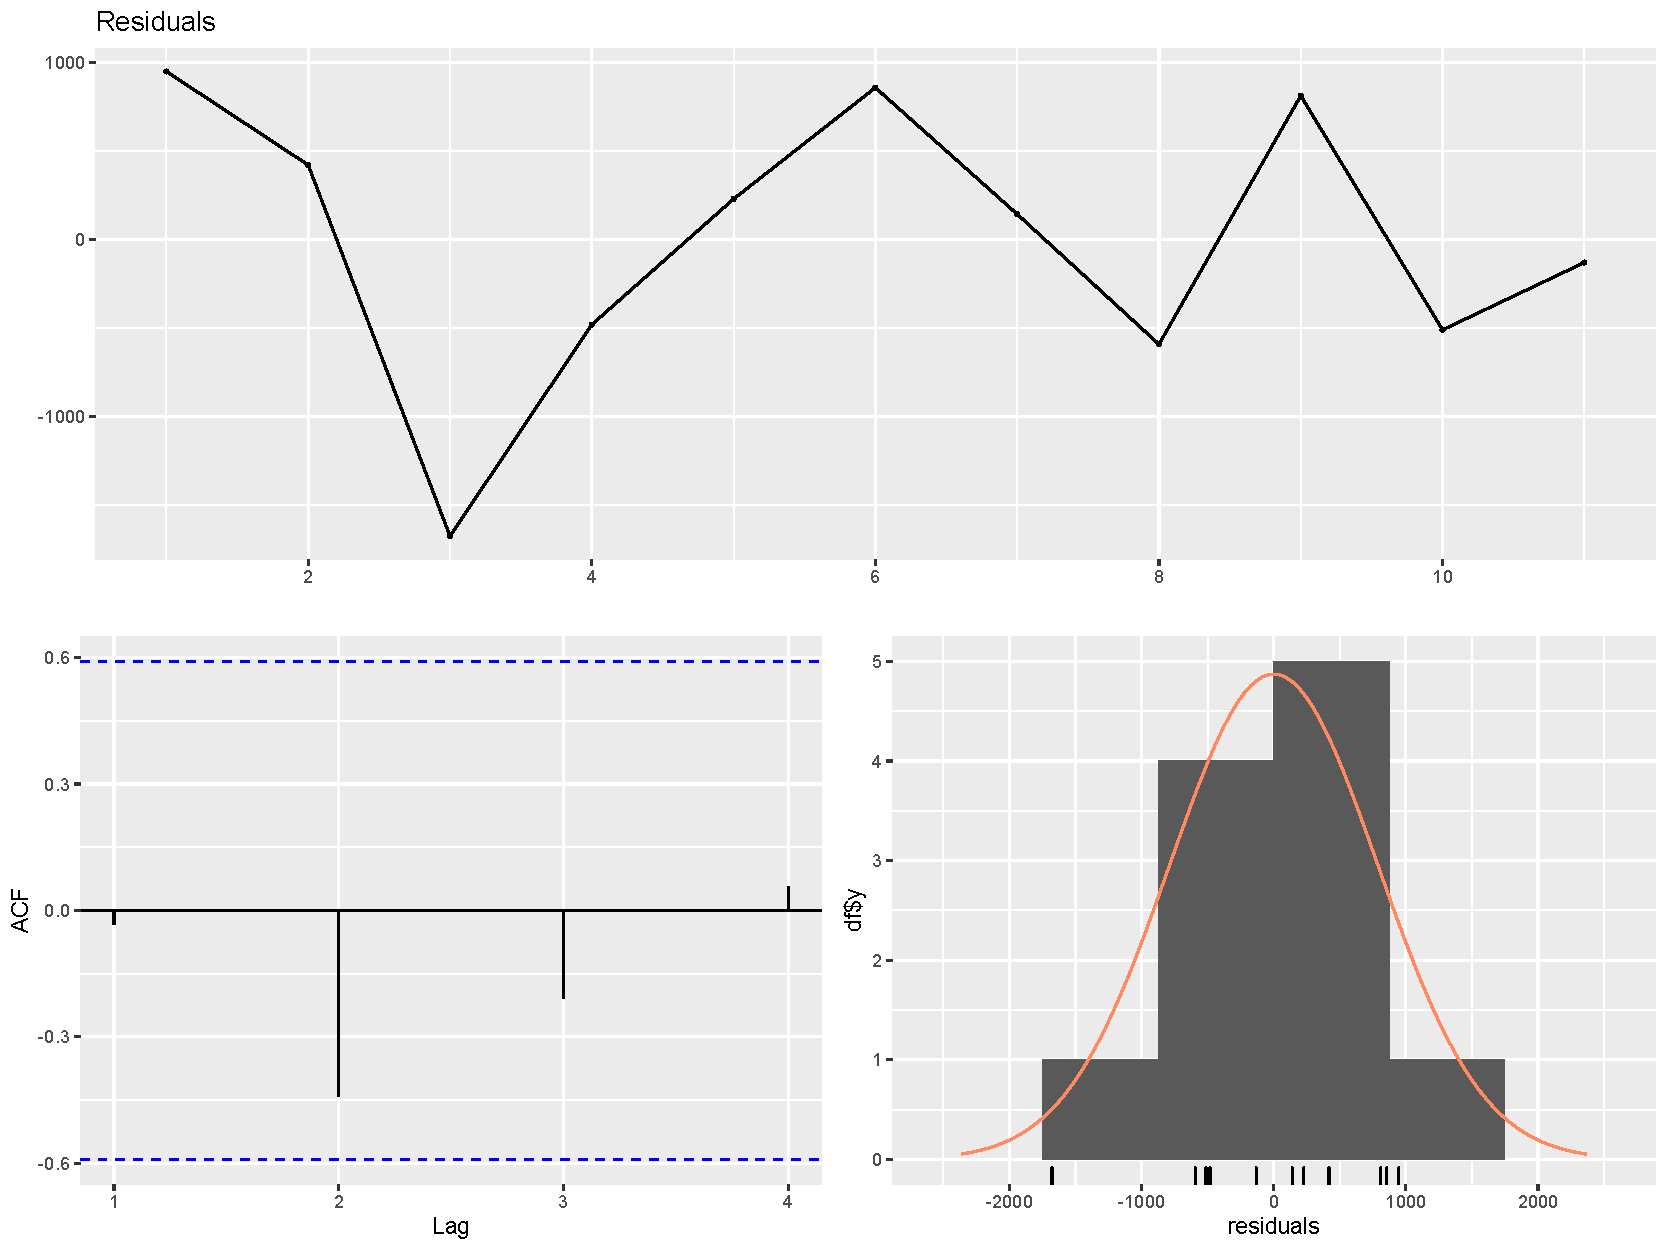
\includegraphics[width=1\textwidth]{loss_model_resi.pdf} %插入图片,[]中设置图片大小,{}中是图片文件名
      \caption{回归结果的残差图} %最终文档中希望显示的图片标题
      \label{loss_model_resi} %用于文内引用的标签
    \end{minipage}
  \end{figure} 
  \subsection{预测2022年的损失}
  假设5月份经济损失有望得到改善,即四月份为损失最严重的时期,那么且疫情不在
  反弹。那么预测从今年三月份开始到年末的社会消费品零售总额损失如下:
  % Table generated by Excel2LaTeX from sheet 'Sheet1'
  \begin{table}[H]
    \centering
    \caption{2022年3月起社会消费品零售总额的损失(单位:亿元)}
      \begin{tabular}{ccccccccccc}
      月份    & 3     & 4     & 5     & 6     & 7     & 8     & 9     & 10    & 11    & 12 \\
      \hline
      损失    & 3924 & 8587 & 6364 & 4735 & 3542 & 2667 & 2026 & 1557 & 1213 & 961 \\
      \end{tabular}%
    \label{loss_2020_table}%
  \end{table}%
  损失的社会消费品零售总额共计35576.72亿元损失,绘出曲线图如下:\nocite{yandou}
  \begin{figure}[H] %H为当前位置,!htb为忽略美学标准,htbp为浮动图形
    \centering %图片居中
    \begin{minipage}[t]{0.4\textwidth}
      \centering
      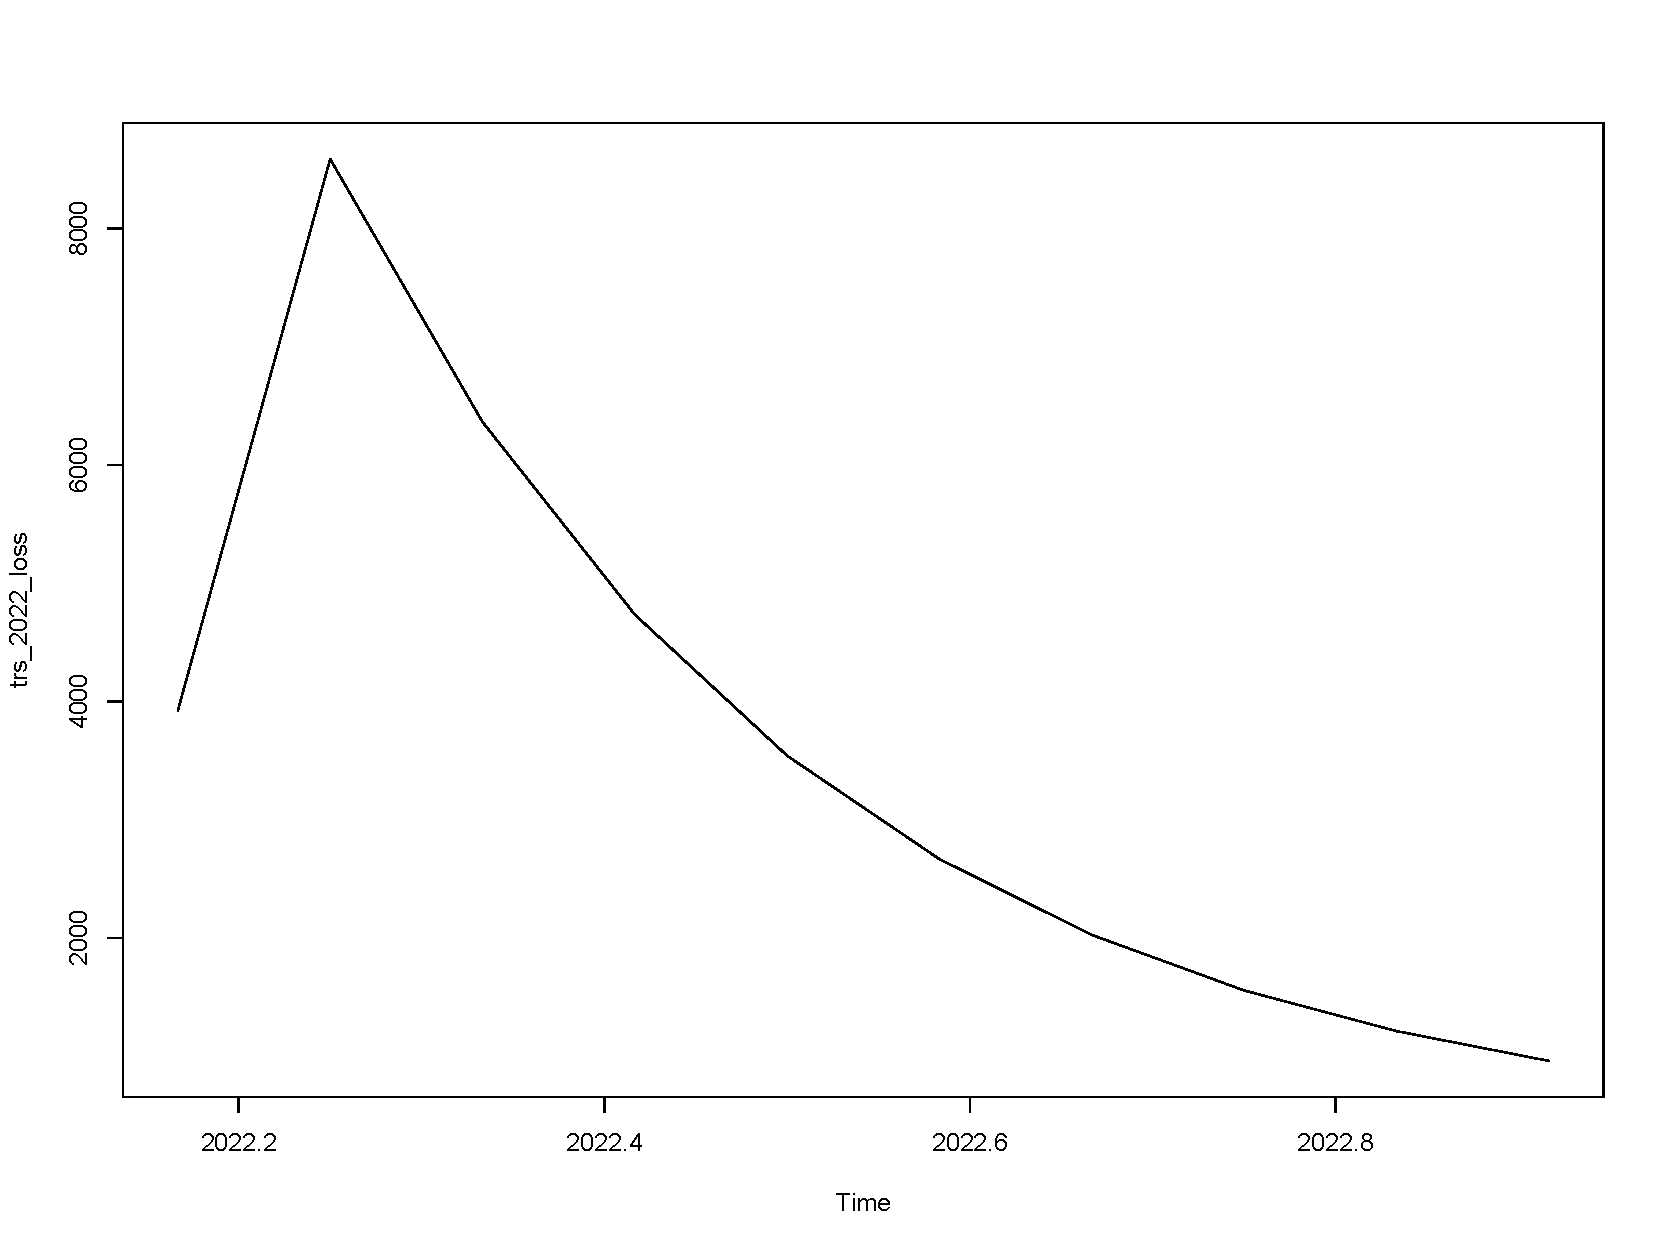
\includegraphics[width=1\textwidth]{loss_2022.pdf} %插入图片,[]中设置图片大小,{}中是图片文件名
      \caption{2022年3月起社会消费品零售总额的损失} %最终文档中希望显示的图片标题
      \label{loss_2022} %用于文内引用的标签
    \end{minipage}
    \begin{minipage}[t]{0.4\textwidth}
      \centering %图片居中
      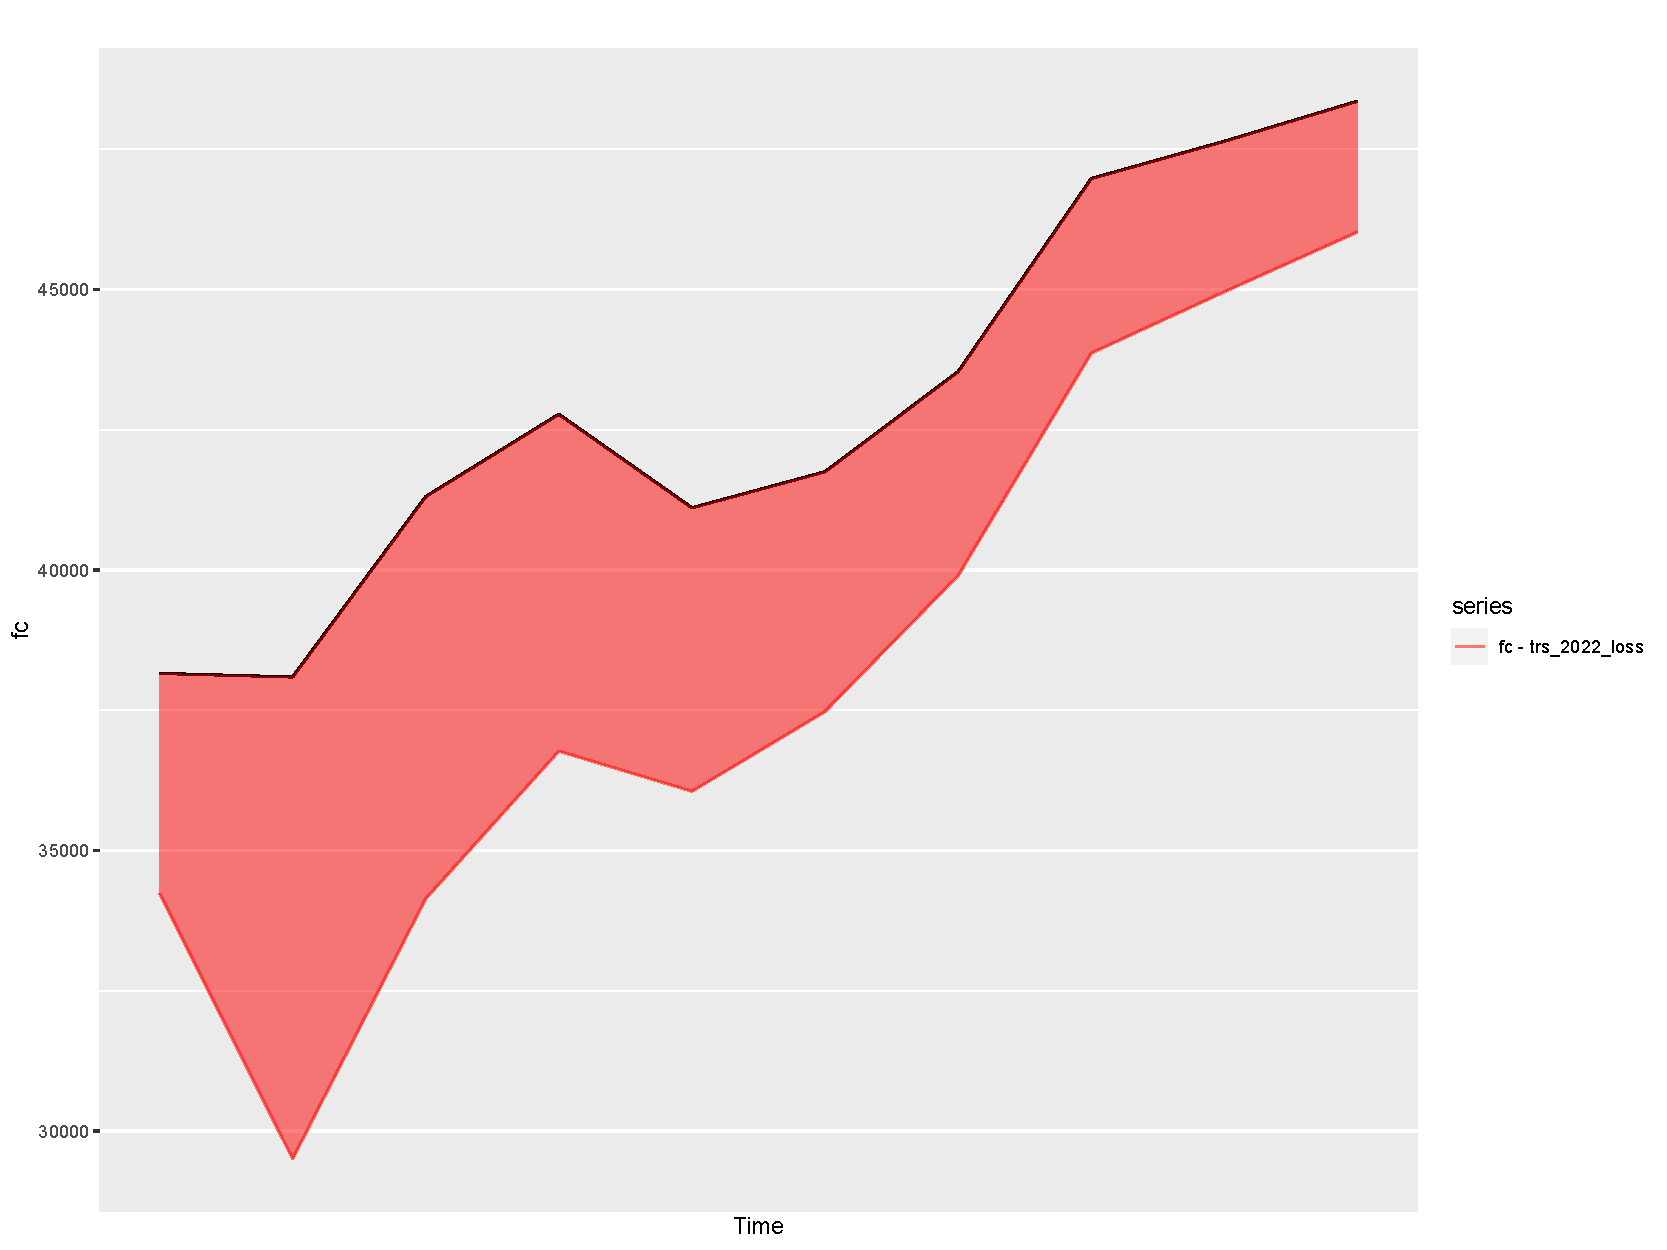
\includegraphics[width=1\textwidth]{compare_2022.pdf} %插入图片,[]中设置图片大小,{}中是图片文件名
      \caption{红色面积为预测损失} %最终文档中希望显示的图片标题
      \label{compare_2022} %用于文内引用的标签
    \end{minipage}
  \end{figure} 
  \section{模型的评价}
  \subsection{优点}
  (1)使用的模型简单,只需通过自身的变量进行建模,不需要依靠过多外部变量
  就能完成建模,减少数据收集的难度

  (2)先对数据进行STL季节性分解,能够对原数据的规律有较为直观的认识,
  发现数据同时具有线性递增和季节波动的特点。

  (3)检验充分,对数据的平稳性和随机性检验,以及多次对模型的残差进行检验,说明模型比较可靠

  (4)在确定\(p,q\)参数时考虑全面,通过网格化枚举的方式,利用AIC, AICc, BIC准则 
  选取最优的模型,一定程度上避免了直接通过ACF和PACF图主观选取参数。

  \subsection{缺点}
  (1) 没有充分的理由假设2020年和2022年疫情对经济的干预相同,
  因此,直接利用通过2020年的干预分析模型预测2022年的经济损失不具有充分说服力。

  (2) ARIMA模型预测的误差会随时间的增加逐渐增大,所以对于10个月的预测
  具有一定的误差存在。
\subsection*{课程学习感悟}
  选择这门课程的主要目的是想了解数学是如何应用于解决生活中的实际问题的。数学建模的基本步骤中
  最重要的两点就是参数估计和假设检验两部分。接着课上介绍很多不同的模型,比如多元分析,
  线性规划,微分方程,还有图论相关的模型。课上比较强调的是线性回归模型。虽然在中学就已经接触最小二乘法求回归直线的问题,
  但是基于此却能衍生出很多的应用,比如机器学习中使用最多的方法之一就是线性回归。
  
  另外通过作业的练习R语言的基本使用。体会到R语言的极大的便利性,首先开源、免费、轻量,
  平时要引进新的package也很方便,package里面的函数功能也很强大,基本上几条命令就能搞定,
  比起其他语言很容易就能上手。

  通过这次大作业也得到了充分的锻炼,从开始的选题,数据收集,编程,到最后写论文,都不断
  的学到了新的知识和技能。学到了很多时间序列分析相关的知识,熟悉时序分析相关的库函数,
  到最后使用Latex撰写论文,最终得到令自己满意的结果。总之,学习这门课感觉收获颇丰,
  希望以后有机会能参加相关的比赛,进一步提高自己建模水平。



\newpage
\bibliographystyle{gbt7714-numerical}
\bibliography{ref.bib}


\newpage
  \begin{center}
    \large{\textbf{Forecast the loss of total retail sales of consumer goods in 2022
     - Based on a seasonal ARIMA model}}


    \textbf{Abstract}
  \end{center}
  

%abstract---------------
{
\setlength{\parindent}{2em}
The total retail sales of social consumer goods(TRS) is an important barometer to measure people's consumption level, and it is also an important barometer in the national economic.
TRS lost in 2022 can be applied to be a key factor of the overall economic loss.

This article first decomposes the STL seasonal decomposition of the previous monthly statistics to obtain the seasonal fluctuations of the time sequence.
After that make a first-order difference on the original time sequence, and then the seasons differential on the sequence of the differential sequence to obtain
a smooth time sequence. Then perform parameter estimation through seasonal Arima models, and
get the prediction value of without epidemic intervention in 2022. Then use the data before 2020 to establish the ARIMA model to obtain the predicted value 
that has not been affected by the epidemic in 2020. Utilize 2020
Forecast values and actual values to do intervention analysis modeling based on epidemic intervention. Then apply the model to get the
predictive value in 2022 during pandemic intervention. Finally, the loss of TRS in 2022 can be forecasted by combining with the prediction value of the Arima model.
Use the R language model and calculate and plot.

\flushleft{\textbf{Keywords:}}total retail sales of social consumer goods ; seasonal ARIMA ;
time series analysis ; intervention analysis


}



\newpage

\begin{appendices}

\section*{}

\textbf{\textcolor[rgb]{0.98,0.00,0.00}{程序一:对原时间序列季节性分解以及数据检验:}}
\lstinputlisting[language=R]{./code/code/TRS_anlanysize.r}

\section*{}

\textcolor[rgb]{0.98,0.00,0.00}{\textbf{程序二:ARIMA模型的选取和预测:}}
\lstinputlisting[language=R]{./code/code/Seasonal_ARIMA.r}

\section*{}

\textcolor[rgb]{0.98,0.00,0.00}{\textbf{程序三:干预分析模型的建立和预测:}}
\lstinputlisting[language=R]{./code/code/intervention.r}

\section*{}

\end{appendices}
\end{document}
%%
%% This work consists of these files mcmthesis.dtx,
%%                                   figures/ and
%%                                   code/,
%% and the derived files             mcmthesis.cls,
%%                                   mcmthesis-demo.tex,
%%                                   README,
%%                                   LICENSE,
%%                                   mcmthesis.pdf and
%%                                   mcmthesis-demo.pdf.
%%
%% End of file `mcmthesis-demo.tex'.
